%%=============================================================================
%% LaTeX sjabloon voor bachelorproef, HoGent Bedrijf en Organisatie
%% Opleiding Toegepaste Informatica
%%=============================================================================

\documentclass[fleqn,a4paper,12pt]{book}

%%=============================================================================
%% LaTeX sjabloon voor de bachelorproef, HoGent Bedrijf en Organisatie
%% Opleiding toegepaste informatica
%%
%% Structuur en algemene vormgeving. Meestal hoef je hier niets te wijzigen.
%%
%% Vormgeving gebaseerd op "The Legrand Orange Book", version 2.0 (9/2/15)
%% door Mathias Legrand (legrand.mathias@gmail.com) met aanpassingen door
%% Vel (vel@latextemplates.com). Het oorspronkelijke template is te vinden op
%% http://www.LaTeXTemplates.com
%%
%% Aanpassingen voor HoGent toegepaste informatica:
%%   Bert Van Vreckem <bert.vanvreckem@hogent.be>
%% Licentie:
%%   CC BY-NC-SA 3.0 (http://creativecommons.org/licenses/by-nc-sa/3.0/)
%%=============================================================================

%%-----------------------------------------------------------------------------
%% Packages
%%-----------------------------------------------------------------------------

\usepackage[top=3cm,bottom=3cm,left=3cm,right=3cm,headsep=10pt,a4paper]{geometry} % Page margins
\usepackage[utf8]{inputenc}  % Accenten gebruiken in tekst (vb. é ipv \'e)
\usepackage{amsfonts}        % AMS math packages: extra wiskundige
\usepackage{amsmath}         %   symbolen (o.a. getallen-
\usepackage{amssymb}         %   verzamelingen N, R, Z, Q, etc.)
\usepackage[english,dutch]{babel}    % Taalinstellingen: woordsplitsingen,
                             %  commando's voor speciale karakters
                             %  ("dutch" voor NL)
\usepackage{iflang}
\usepackage{eurosym}         % Euro-symbool €
\usepackage{geometry}
\usepackage{graphicx}        % Invoegen van tekeningen
\graphicspath{{img/}}       % Specifies the directory where pictures are stored
\usepackage{tikz}            % Required for drawing custom shapes
\usepackage[pdftex,bookmarks=true]{hyperref}
                             % PDF krijgt klikbare links & verwijzingen,
                             %  inhoudstafel
\usepackage{enumitem}        % Customize lists
\setlist{nolistsep}         % Reduce spacing between list items
\usepackage{listings}        % Broncode mooi opmaken
\usepackage{multirow}        % Tekst over verschillende cellen in tabellen
\usepackage{rotating}        % Tabellen en figuren roteren

%custom
\usepackage{float}
\usepackage{pgfplots}

\usepackage{booktabs}        % Required for nicer horizontal rules in tables

\usepackage{xcolor}          % Required for specifying colors by name
\definecolor{maincolor}{RGB}{0,147,208} % Define the main color used for
                             % highlighting throughout the book
                             % 0, 147, 208 = officiële kleur HoGent FBO

% Paragraph style: no indent, add space between paragraphs
\setlength{\parindent}{0em}
\setlength{\parskip}{1em}

\usepackage{etoolbox}
\usepackage{titling} % Macros for title, author, etc
\usepackage{lipsum}          % Voor vultekst (lorem ipsum)

%----------------------------------------------------------------------------------------
%	FONTS
%----------------------------------------------------------------------------------------

\usepackage{avant} % Use the Avantgarde font for headings
%\usepackage{times} % Use the Times font for headings
\usepackage{mathptmx} % Use the Adobe Times Roman as the default text font together with math symbols from the Sym­bol, Chancery and Com­puter Modern fonts

\usepackage{microtype} % Slightly tweak font spacing for aesthetics
\usepackage[utf8]{inputenc} % Required for including letters with accents
\usepackage[T1]{fontenc} % Use 8-bit encoding that has 256 glyphs

%------------------------------------------------------------------------------
%	TITLE PAGE
%------------------------------------------------------------------------------

\newcommand{\inserttitlepage}{%
\begin{titlepage}
  \newgeometry{top=2cm,bottom=1.5cm,left=1.5cm,right=1.5cm}
  \begin{center}

    \begingroup
    \rmfamily
    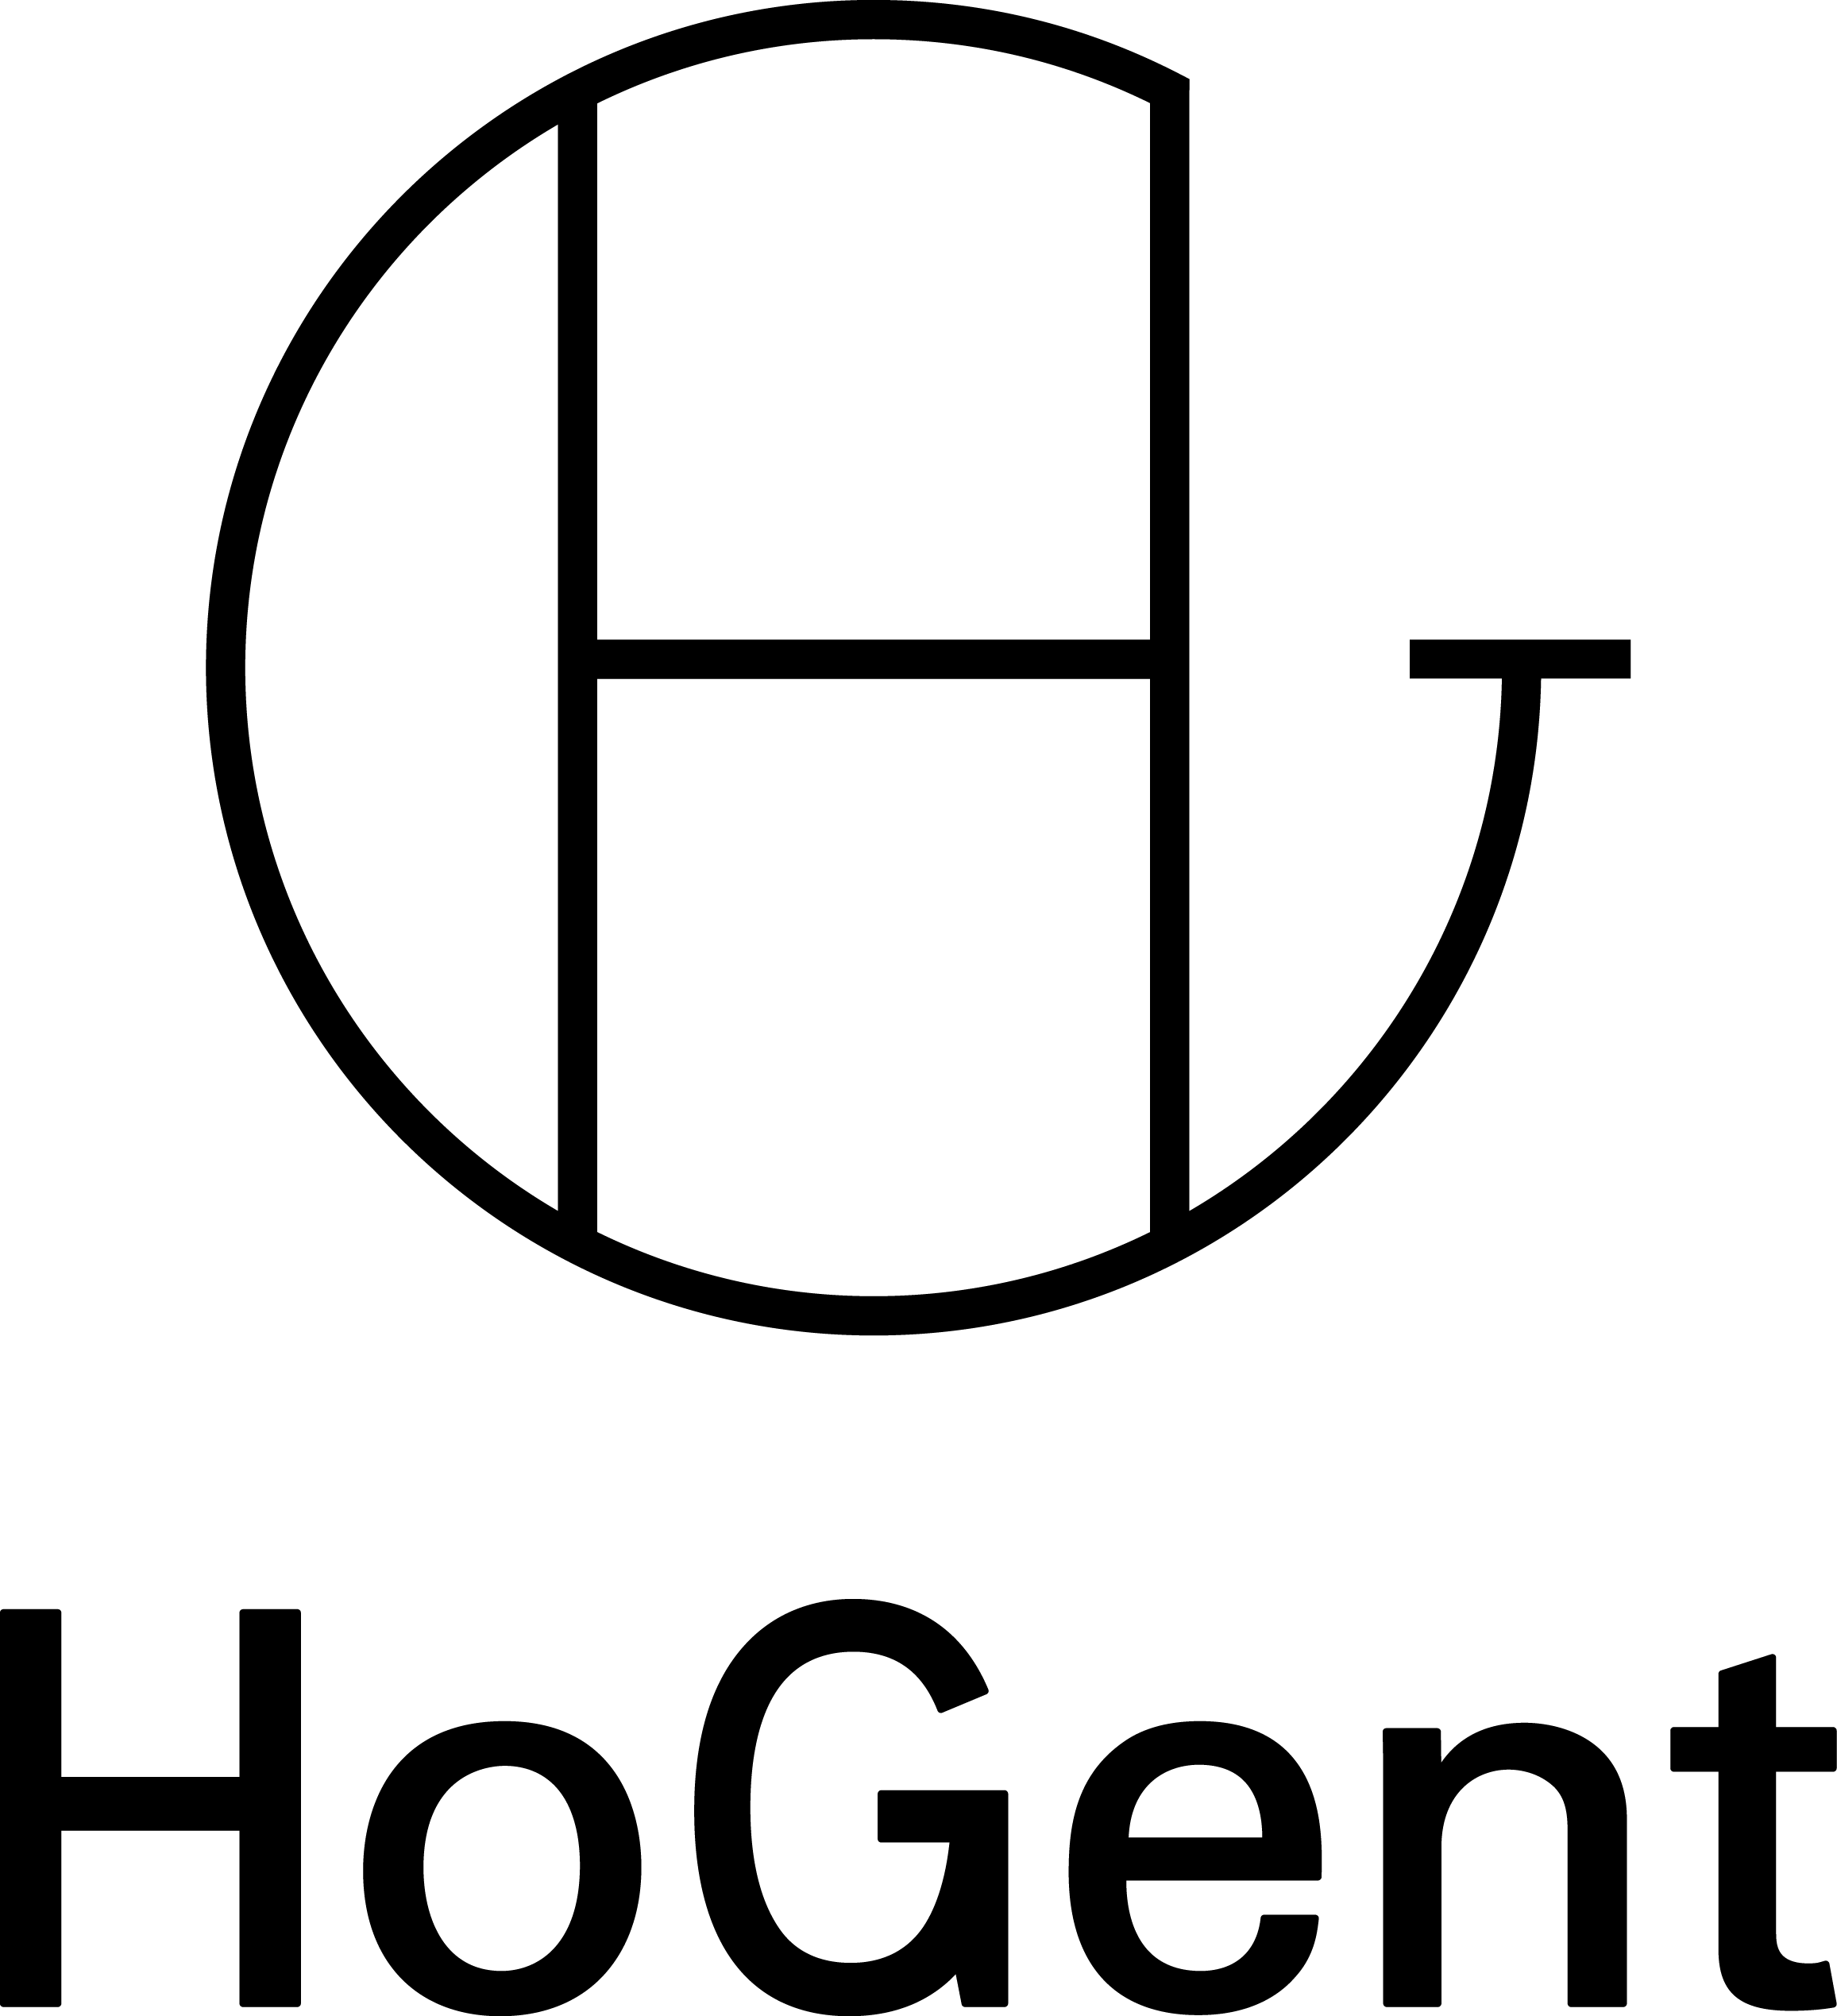
\includegraphics[width=2.5cm]{img/HG-beeldmerk-woordmerk}\\[.5cm]
    Faculteit Bedrijf en Organisatie\\[3cm]
    \titel
    \vfill
    \student\\[3.5cm]
    Scriptie voorgedragen tot het bekomen van de graad van\\professionele bachelor in de toegepaste informatica\\[2cm]
    Promotor:\\
    \promotor\\
    \ifdefempty{\copromotor}{\vspace{2.5cm}}{Co-promotor:\\\copromotor\\[2.5cm]}
    Instelling: \instelling\\[.5cm]
    Academiejaar: \academiejaar\\[.5cm]
    \ifcase \examenperiode \or Eerste \or Tweede \else Derde \fi examenperiode
    \endgroup

  \end{center}
  \restoregeometry
\end{titlepage}
  \emptypage
\begin{titlepage}
  \newgeometry{top=5.35cm,bottom=1.5cm,left=1.5cm,right=1.5cm}
  \begin{center}

    \begingroup
    \rmfamily
    \IfLanguageName{dutch}{Faculteit Bedrijf en Organisatie}{Faculty of Business and Information Management}\\[3cm]
    \titel
    \vfill
    \student\\[3.5cm]
    \IfLanguageName{dutch}{Scriptie voorgedragen tot het bekomen van de graad van\\professionele bachelor in de toegepaste informatica}{Thesis submitted in partial fulfillment of the requirements for the degree of\\professional bachelor of applied computer science}\\[2cm]
    Promotor:\\
    \promotor\\
    \ifdefempty{\copromotor}{\vspace{2.5cm}}{Co-promotor:\\\copromotor\\[2.5cm]}
    \IfLanguageName{dutch}{Instelling}{Institution}: \instelling\\[.5cm]
    \IfLanguageName{dutch}{Academiejaar}{Academic year}: \academiejaar\\[.5cm]
    \IfLanguageName{dutch}{%
    \ifcase \examenperiode \or Eerste \or Tweede \else Derde \fi examenperiode}{%
    \ifcase \examenperiode \or First \or Second \else Third \fi examination period}
    \endgroup

  \end{center}
  \restoregeometry
\end{titlepage}
}

%----------------------------------------------------------------------------------------
%	BIBLIOGRAPHY AND INDEX
%----------------------------------------------------------------------------------------

\usepackage[style=apa,backend=biber]{biblatex}
\usepackage{csquotes}
\DeclareLanguageMapping{dutch}{dutch-apa}
\addbibresource{bachproef-tin.bib} % BibTeX bibliography file
\defbibheading{bibempty}{}

\usepackage{calc} % For simpler calculation - used for spacing the index letter headings correctly
\usepackage{makeidx} % Required to make an index
\makeindex % Tells LaTeX to create the files required for indexing

%----------------------------------------------------------------------------------------
%	MAIN TABLE OF CONTENTS
%----------------------------------------------------------------------------------------

\usepackage{titletoc} % Required for manipulating the table of contents

\contentsmargin{0cm} % Removes the default margin

% Part text styling
\titlecontents{part}[0cm]
{\addvspace{20pt}\centering\large\bfseries}
{}
{}
{}

% Chapter text styling
\titlecontents{chapter}[1.25cm] % Indentation
{\addvspace{12pt}\large\sffamily\bfseries} % Spacing and font options for chapters
{\color{maincolor!60}\contentslabel[\Large\thecontentslabel]{1.25cm}\color{maincolor}} % Chapter number
{\color{maincolor}}
{\color{maincolor!60}\normalsize\;\titlerule*[.5pc]{.}\;\thecontentspage} % Page number

% Section text styling
\titlecontents{section}[1.25cm] % Indentation
{\addvspace{3pt}\sffamily\bfseries} % Spacing and font options for sections
{\contentslabel[\thecontentslabel]{1.25cm}} % Section number
{}
{\hfill\color{black}\thecontentspage} % Page number
[]

% Subsection text styling
\titlecontents{subsection}[1.25cm] % Indentation
{\addvspace{1pt}\sffamily\small} % Spacing and font options for subsections
{\contentslabel[\thecontentslabel]{1.25cm}} % Subsection number
{}
{\ \titlerule*[.5pc]{.}\;\thecontentspage} % Page number
[]

% List of figures
\titlecontents{figure}[0em]
{\addvspace{-5pt}\sffamily}
{\thecontentslabel\hspace*{1em}}
{}
{\ \titlerule*[.5pc]{.}\;\thecontentspage}
[]

% List of tables
\titlecontents{table}[0em]
{\addvspace{-5pt}\sffamily}
{\thecontentslabel\hspace*{1em}}
{}
{\ \titlerule*[.5pc]{.}\;\thecontentspage}
[]

%----------------------------------------------------------------------------------------
%	MINI TABLE OF CONTENTS IN PART HEADS
%----------------------------------------------------------------------------------------

% Chapter text styling
\titlecontents{lchapter}[0em] % Indenting
{\addvspace{15pt}\large\sffamily\bfseries} % Spacing and font options for chapters
{\color{maincolor}\contentslabel[\Large\thecontentslabel]{1.25cm}\color{maincolor}} % Chapter number
{}
{\color{maincolor}\normalsize\sffamily\bfseries\;\titlerule*[.5pc]{.}\;\thecontentspage} % Page number

% Section text styling
\titlecontents{lsection}[0em] % Indenting
{\sffamily\small} % Spacing and font options for sections
{\contentslabel[\thecontentslabel]{1.25cm}} % Section number
{}
{}

% Subsection text styling
\titlecontents{lsubsection}[.5em] % Indentation
{\normalfont\footnotesize\sffamily} % Font settings
{}
{}
{}

%----------------------------------------------------------------------------------------
%	PAGE HEADERS
%----------------------------------------------------------------------------------------

\usepackage{fancyhdr} % Required for header and footer configuration

\pagestyle{fancy}
\renewcommand{\chaptermark}[1]{\markboth{\sffamily\normalsize\bfseries\chaptername\ \thechapter.\ #1}{}} % Chapter text font settings
\renewcommand{\sectionmark}[1]{\markright{\sffamily\normalsize\thesection\hspace{5pt}#1}{}} % Section text font settings
\fancyhf{} \fancyhead[LE,RO]{\sffamily\normalsize\thepage} % Font setting for the page number in the header
\fancyhead[LO]{\rightmark} % Print the nearest section name on the left side of odd pages
\fancyhead[RE]{\leftmark} % Print the current chapter name on the right side of even pages
\renewcommand{\headrulewidth}{0.5pt} % Width of the rule under the header
\addtolength{\headheight}{2.5pt} % Increase the spacing around the header slightly
\renewcommand{\footrulewidth}{0pt} % Removes the rule in the footer
\fancypagestyle{plain}{\fancyhead{}\renewcommand{\headrulewidth}{0pt}} % Style for when a plain pagestyle is specified

% Removes the header from odd empty pages at the end of chapters
\makeatletter
\renewcommand{\cleardoublepage}{
\clearpage\ifodd\c@page\else
\hbox{}
\vspace*{\fill}
\thispagestyle{empty}
\newpage
\fi}

%----------------------------------------------------------------------------------------
%	THEOREM STYLES
%----------------------------------------------------------------------------------------

\usepackage{amsmath,amsfonts,amssymb,amsthm} % For math equations, theorems, symbols, etc

\newcommand{\intoo}[2]{\mathopen{]}#1\,;#2\mathclose{[}}
\newcommand{\ud}{\mathop{\mathrm{{}d}}\mathopen{}}
\newcommand{\intff}[2]{\mathopen{[}#1\,;#2\mathclose{]}}
\newtheorem{notation}{Notation}[chapter]

% Boxed/framed environments
\newtheoremstyle{maincolornumbox}% % Theorem style name
{0pt}% Space above
{0pt}% Space below
{\normalfont}% % Body font
{}% Indent amount
{\small\bf\sffamily\color{maincolor}}% % Theorem head font
{\;}% Punctuation after theorem head
{0.25em}% Space after theorem head
{\small\sffamily\color{maincolor}\thmname{#1}\nobreakspace\thmnumber{\@ifnotempty{#1}{}\@upn{#2}}% Theorem text (e.g. Theorem 2.1)
\thmnote{\nobreakspace\the\thm@notefont\sffamily\bfseries\color{black}---\nobreakspace#3.}} % Optional theorem note
\renewcommand{\qedsymbol}{$\blacksquare$}% Optional qed square

\newtheoremstyle{blacknumex}% Theorem style name
{5pt}% Space above
{5pt}% Space below
{\normalfont}% Body font
{} % Indent amount
{\small\bf\sffamily}% Theorem head font
{\;}% Punctuation after theorem head
{0.25em}% Space after theorem head
{\small\sffamily{\tiny\ensuremath{\blacksquare}}\nobreakspace\thmname{#1}\nobreakspace\thmnumber{\@ifnotempty{#1}{}\@upn{#2}}% Theorem text (e.g. Theorem 2.1)
\thmnote{\nobreakspace\the\thm@notefont\sffamily\bfseries---\nobreakspace#3.}}% Optional theorem note

\newtheoremstyle{blacknumbox} % Theorem style name
{0pt}% Space above
{0pt}% Space below
{\normalfont}% Body font
{}% Indent amount
{\small\bf\sffamily}% Theorem head font
{\;}% Punctuation after theorem head
{0.25em}% Space after theorem head
{\small\sffamily\thmname{#1}\nobreakspace\thmnumber{\@ifnotempty{#1}{}\@upn{#2}}% Theorem text (e.g. Theorem 2.1)
\thmnote{\nobreakspace\the\thm@notefont\sffamily\bfseries---\nobreakspace#3.}}% Optional theorem note

% Non-boxed/non-framed environments
\newtheoremstyle{maincolornum}% % Theorem style name
{5pt}% Space above
{5pt}% Space below
{\normalfont}% % Body font
{}% Indent amount
{\small\bf\sffamily\color{maincolor}}% % Theorem head font
{\;}% Punctuation after theorem head
{0.25em}% Space after theorem head
{\small\sffamily\color{maincolor}\thmname{#1}\nobreakspace\thmnumber{\@ifnotempty{#1}{}\@upn{#2}}% Theorem text (e.g. Theorem 2.1)
\thmnote{\nobreakspace\the\thm@notefont\sffamily\bfseries\color{black}---\nobreakspace#3.}} % Optional theorem note
\renewcommand{\qedsymbol}{$\blacksquare$}% Optional qed square
\makeatother

% Defines the theorem text style for each type of theorem to one of the three styles above
\newcounter{dummy}
\numberwithin{dummy}{section}
\theoremstyle{maincolornumbox}
\newtheorem{theoremeT}[dummy]{Theorem}
\newtheorem{problem}{Problem}[chapter]
\newtheorem{exerciseT}{Exercise}[chapter]
\theoremstyle{blacknumex}
\newtheorem{exampleT}{Example}[chapter]
\theoremstyle{blacknumbox}
\newtheorem{vocabulary}{Vocabulary}[chapter]
\newtheorem{definitionT}{Definition}[section]
\newtheorem{corollaryT}[dummy]{Corollary}
\theoremstyle{maincolornum}
\newtheorem{proposition}[dummy]{Proposition}

%----------------------------------------------------------------------------------------
%	DEFINITION OF COLORED BOXES
%----------------------------------------------------------------------------------------

\RequirePackage[framemethod=default]{mdframed} % Required for creating the theorem, definition, exercise and corollary boxes

% Theorem box
\newmdenv[skipabove=7pt,
skipbelow=7pt,
backgroundcolor=black!5,
linecolor=maincolor,
innerleftmargin=5pt,
innerrightmargin=5pt,
innertopmargin=5pt,
leftmargin=0cm,
rightmargin=0cm,
innerbottommargin=5pt]{tBox}

% Exercise box
\newmdenv[skipabove=7pt,
skipbelow=7pt,
rightline=false,
leftline=true,
topline=false,
bottomline=false,
backgroundcolor=maincolor!10,
linecolor=maincolor,
innerleftmargin=5pt,
innerrightmargin=5pt,
innertopmargin=5pt,
innerbottommargin=5pt,
leftmargin=0cm,
rightmargin=0cm,
linewidth=4pt]{eBox}

% Definition box
\newmdenv[skipabove=7pt,
skipbelow=7pt,
rightline=false,
leftline=true,
topline=false,
bottomline=false,
linecolor=maincolor,
innerleftmargin=5pt,
innerrightmargin=5pt,
innertopmargin=0pt,
leftmargin=0cm,
rightmargin=0cm,
linewidth=4pt,
innerbottommargin=0pt]{dBox}

% Corollary box
\newmdenv[skipabove=7pt,
skipbelow=7pt,
rightline=false,
leftline=true,
topline=false,
bottomline=false,
linecolor=gray,
backgroundcolor=black!5,
innerleftmargin=5pt,
innerrightmargin=5pt,
innertopmargin=5pt,
leftmargin=0cm,
rightmargin=0cm,
linewidth=4pt,
innerbottommargin=5pt]{cBox}

% Creates an environment for each type of theorem and assigns it a theorem text style from the "Theorem Styles" section above and a colored box from above
\newenvironment{theorem}{\begin{tBox}\begin{theoremeT}}{\end{theoremeT}\end{tBox}}
\newenvironment{exercise}{\begin{eBox}\begin{exerciseT}}{\hfill{\color{maincolor}\tiny\ensuremath{\blacksquare}}\end{exerciseT}\end{eBox}}
\newenvironment{definition}{\begin{dBox}\begin{definitionT}}{\end{definitionT}\end{dBox}}
\newenvironment{example}{\begin{exampleT}}{\hfill{\tiny\ensuremath{\blacksquare}}\end{exampleT}}
\newenvironment{corollary}{\begin{cBox}\begin{corollaryT}}{\end{corollaryT}\end{cBox}}

%----------------------------------------------------------------------------------------
%	REMARK ENVIRONMENT
%----------------------------------------------------------------------------------------

\newenvironment{remark}{\par\vspace{10pt}\small % Vertical white space above the remark and smaller font size
\begin{list}{}{
\leftmargin=35pt % Indentation on the left
\rightmargin=25pt}\item\ignorespaces % Indentation on the right
\makebox[-2.5pt]{\begin{tikzpicture}[overlay]
\node[draw=maincolor!60,line width=1pt,circle,fill=maincolor!25,font=\sffamily\bfseries,inner sep=2pt,outer sep=0pt] at (-15pt,0pt){\textcolor{maincolor}{R}};\end{tikzpicture}} % Orange R in a circle
\advance\baselineskip -1pt}{\end{list}\vskip5pt} % Tighter line spacing and white space after remark

%----------------------------------------------------------------------------------------
%	SECTION NUMBERING IN THE MARGIN
%----------------------------------------------------------------------------------------

\makeatletter
\renewcommand{\@seccntformat}[1]{\llap{\textcolor{maincolor}{\csname the#1\endcsname}\hspace{1em}}}
\renewcommand{\section}{\@startsection{section}{1}{\z@}
{-4ex \@plus -1ex \@minus -.4ex}
{1ex \@plus.2ex }
{\normalfont\large\sffamily\bfseries}}
\renewcommand{\subsection}{\@startsection {subsection}{2}{\z@}
{-3ex \@plus -0.1ex \@minus -.4ex}
{0.5ex \@plus.2ex }
{\normalfont\sffamily\bfseries}}
\renewcommand{\subsubsection}{\@startsection {subsubsection}{3}{\z@}
{-2ex \@plus -0.1ex \@minus -.2ex}
{.2ex \@plus.2ex }
{\normalfont\small\sffamily\bfseries}}
\renewcommand\paragraph{\@startsection{paragraph}{4}{\z@}
{-2ex \@plus-.2ex \@minus .2ex}
{.1ex}
{\normalfont\small\sffamily\bfseries}}

%----------------------------------------------------------------------------------------
%	PART HEADINGS
%----------------------------------------------------------------------------------------

% numbered part in the table of contents
\newcommand{\@mypartnumtocformat}[2]{%
\setlength\fboxsep{0pt}%
\noindent\colorbox{maincolor!20}{\strut\parbox[c][.7cm]{\ecart}{\color{maincolor!70}\Large\sffamily\bfseries\centering#1}}\hskip\esp\colorbox{maincolor!40}{\strut\parbox[c][.7cm]{\linewidth-\ecart-\esp}{\Large\sffamily\centering#2}}}%
%%%%%%%%%%%%%%%%%%%%%%%%%%%%%%%%%%
% unnumbered part in the table of contents
\newcommand{\@myparttocformat}[1]{%
\setlength\fboxsep{0pt}%
\noindent\colorbox{maincolor!40}{\strut\parbox[c][.7cm]{\linewidth}{\Large\sffamily\centering#1}}}%
%%%%%%%%%%%%%%%%%%%%%%%%%%%%%%%%%%
\newlength\esp
\setlength\esp{4pt}
\newlength\ecart
\setlength\ecart{1.2cm-\esp}
\newcommand{\thepartimage}{}%
\newcommand{\partimage}[1]{\renewcommand{\thepartimage}{#1}}%
\def\@part[#1]#2{%
\ifnum \c@secnumdepth >-2\relax%
\refstepcounter{part}%
\addcontentsline{toc}{part}{\texorpdfstring{\protect\@mypartnumtocformat{\thepart}{#1}}{\partname~\thepart\ ---\ #1}}
\else%
\addcontentsline{toc}{part}{\texorpdfstring{\protect\@myparttocformat{#1}}{#1}}%
\fi%
\startcontents%
\markboth{}{}%
{\thispagestyle{empty}%
\begin{tikzpicture}[remember picture,overlay]%
\node at (current page.north west){\begin{tikzpicture}[remember picture,overlay]%
\fill[maincolor!20](0cm,0cm) rectangle (\paperwidth,-\paperheight);
\node[anchor=north] at (4cm,-3.25cm){\color{maincolor!40}\fontsize{220}{100}\sffamily\bfseries\@Roman\c@part};
\node[anchor=south east] at (\paperwidth-1cm,-\paperheight+1cm){\parbox[t][][t]{8.5cm}{
\printcontents{l}{0}{\setcounter{tocdepth}{1}}%
}};
\node[anchor=north east] at (\paperwidth-1.5cm,-3.25cm){\parbox[t][][t]{15cm}{\strut\raggedleft\color{white}\fontsize{30}{30}\sffamily\bfseries#2}};
\end{tikzpicture}};
\end{tikzpicture}}%
\@endpart}
\def\@spart#1{%
\startcontents%
\phantomsection
{\thispagestyle{empty}%
\begin{tikzpicture}[remember picture,overlay]%
\node at (current page.north west){\begin{tikzpicture}[remember picture,overlay]%
\fill[maincolor!20](0cm,0cm) rectangle (\paperwidth,-\paperheight);
\node[anchor=north east] at (\paperwidth-1.5cm,-3.25cm){\parbox[t][][t]{15cm}{\strut\raggedleft\color{white}\fontsize{30}{30}\sffamily\bfseries#1}};
\end{tikzpicture}};
\end{tikzpicture}}
\addcontentsline{toc}{part}{\texorpdfstring{%
\setlength\fboxsep{0pt}%
\noindent\protect\colorbox{maincolor!40}{\strut\protect\parbox[c][.7cm]{\linewidth}{\Large\sffamily\protect\centering #1\quad\mbox{}}}}{#1}}%
\@endpart}
\def\@endpart{\vfil\newpage
\if@twoside
\if@openright
\null
\thispagestyle{empty}%
\newpage
\fi
\fi
\if@tempswa
\twocolumn
\fi}

%----------------------------------------------------------------------------------------
%	CHAPTER HEADINGS
%----------------------------------------------------------------------------------------

% A switch to conditionally include a picture, implemented by  Christian Hupfer
\newif\ifusechapterimage
\usechapterimagetrue
\newcommand{\thechapterimage}{}%
\newcommand{\chapterimage}[1]{\ifusechapterimage\renewcommand{\thechapterimage}{#1}\fi}%
\def\@makechapterhead#1{%
{\parindent \z@ \raggedright \normalfont
\ifnum \c@secnumdepth >\m@ne
\if@mainmatter
\begin{tikzpicture}[remember picture,overlay]
\node at (current page.north west)
{\begin{tikzpicture}[remember picture,overlay]
\node[anchor=north west,inner sep=0pt] at (0,0) {\ifusechapterimage\includegraphics[width=\paperwidth]{\thechapterimage}\fi};
\draw[anchor=west] (\Gm@lmargin,-9cm) node [line width=2pt,rounded corners=15pt,draw=maincolor,fill=white,fill opacity=0.5,inner sep=15pt]{\strut\makebox[22cm]{}};
\draw[anchor=west] (\Gm@lmargin+.3cm,-9cm) node {\huge\sffamily\bfseries\color{black}\thechapter. #1\strut};
\end{tikzpicture}};
\end{tikzpicture}
\else
\begin{tikzpicture}[remember picture,overlay]
\node at (current page.north west)
{\begin{tikzpicture}[remember picture,overlay]
\node[anchor=north west,inner sep=0pt] at (0,0) {\ifusechapterimage\includegraphics[width=\paperwidth]{\thechapterimage}\fi};
\draw[anchor=west] (\Gm@lmargin,-9cm) node [line width=2pt,rounded corners=15pt,draw=maincolor,fill=white,fill opacity=0.5,inner sep=15pt]{\strut\makebox[22cm]{}};
\draw[anchor=west] (\Gm@lmargin+.3cm,-9cm) node {\huge\sffamily\bfseries\color{black}#1\strut};
\end{tikzpicture}};
\end{tikzpicture}
\fi\fi\par\vspace*{270\p@}}}

%-------------------------------------------

\def\@makeschapterhead#1{%
\begin{tikzpicture}[remember picture,overlay]
\node at (current page.north west)
{\begin{tikzpicture}[remember picture,overlay]
\node[anchor=north west,inner sep=0pt] at (0,0) {\ifusechapterimage\includegraphics[width=\paperwidth]{\thechapterimage}\fi};
\draw[anchor=west] (\Gm@lmargin,-9cm) node [line width=2pt,rounded corners=15pt,draw=maincolor,fill=white,fill opacity=0.5,inner sep=15pt]{\strut\makebox[22cm]{}};
\draw[anchor=west] (\Gm@lmargin+.3cm,-9cm) node {\huge\sffamily\bfseries\color{black}#1\strut};
\end{tikzpicture}};
\end{tikzpicture}
\par\vspace*{270\p@}}
\makeatother

%----------------------------------------------------------------------------------------
%	HYPERLINKS IN THE DOCUMENTS
%----------------------------------------------------------------------------------------

\usepackage{hyperref}
\hypersetup{hidelinks,backref=true,pagebackref=true,hyperindex=true,colorlinks=false,breaklinks=true,urlcolor= maincolor,bookmarks=true,bookmarksopen=false,pdftitle={Title},pdfauthor={Author}}
\usepackage{bookmark}
\bookmarksetup{
open,
numbered,
addtohook={%
\ifnum\bookmarkget{level}=0 % chapter
\bookmarksetup{bold}%
\fi
\ifnum\bookmarkget{level}=-1 % part
\bookmarksetup{color=maincolor,bold}%
\fi
}
}

%----------------------------------------------------------------------------------------
%	Java source code
%----------------------------------------------------------------------------------------

% Commando voor invoegen Java-broncodebestanden (dank aan Niels Corneille)
% Gebruik:
%   \codefragment{source/MijnKlasse.java}{Uitleg bij de code}
%
% Je kan dit aanpassen aan de taal die je zelf het meeste gebruikt in je
% bachelorproef.
\newcommand{\codefragment}[2]{ \lstset{%
  language=java,
  breaklines=true,
  float=th,
  caption={#2},
  basicstyle=\scriptsize,
  frame=single,
  extendedchars=\true
}
\lstinputlisting{#1}}

% Leeg blad
\newcommand{\emptypage}{%
\newpage
\thispagestyle{empty}
\mbox{}
\newpage
}


%%---------- Documenteigenschappen --------------------------------------------
%% TODO: Vul dit aan met je eigen info:

% Je eigen naam
\newcommand{\student}{Matthias Kunnen}

% De naam van je promotor (lector van de opleiding)
\newcommand{\promotor}{Marc Van Asselberg}

% De naam van je co-promotor. Als je promotor ook je opdrachtgever is en je
% dus ook inhoudelijk begeleidt (en enkel dan!), mag je dit leeg laten.
\newcommand{\copromotor}{Tom Van den Bulcke}

% Indien je bachelorproef in opdracht van/in samenwerking met een bedrijf of
% externe organisatie geschreven is, geef je hier de naam. Zoniet laat je dit
% zoals het is.
\newcommand{\instelling}{---}

% De titel van het rapport/bachelorproef
\newcommand{\titel}{Onderzoek naar  fraudegevoeligheid in bedrijven en een mogelijke oplossing door het verzekeren van authenticiteit, integriteit en toerekenbaarheid}

% Datum van indienen (gebruik telkens de deadline, ook al geef je eerder af)
\newcommand{\datum}{9 juni 2017}

% Academiejaar
\newcommand{\academiejaar}{2016-2017}

% Examenperiode
%  - 1e semester = 1e examenperiode => 1
%  - 2e semester = 2e examenperiode => 2
%  - tweede zit  = 3e examenperiode => 3
\newcommand{\examenperiode}{2}

%%=============================================================================
%% Inhoud document
%%=============================================================================

\usepackage{pdfpages}
\expandafter\def\expandafter\UrlBreaks\expandafter{\UrlBreaks%  save the
%current one
	\do\a\do\b\do\c\do\d\do\e\do\f\do\g\do\h\do\i\do\j%
	\do\k\do\l\do\m\do\n\do\o\do\p\do\q\do\r\do\s\do\t%
	\do\u\do\v\do\w\do\x\do\y\do\z\do\A\do\B\do\C\do\D%
	\do\E\do\F\do\G\do\H\do\I\do\J\do\K\do\L\do\M\do\N%
	\do\O\do\P\do\Q\do\R\do\S\do\T\do\U\do\V\do\W\do\X%
	\do\Y\do\Z}

%One single link
\newcommand*{\fullref}[1]{\hyperref[{#1}]{\ref*{#1}:~\textit{\nameref*{#1}}}}

\begin{document}

%---------- Taalselectie ------------------------------------------------------
%% Als je je bachelorproef in het Engels schrijft, haal dan onderstaande regel
%% uit commentaar. Let op: de tekst op de voorkaft blijft in het Nederlands, en
%% dat is ook de bedoeling!
%\selectlanguage{english}

%---------- Titelblad ---------------------------------------------------------
\inserttitlepage

%---------- Samenvatting, voorwoord -------------------------------------------
\usechapterimagefalse
%%=============================================================================
%% Samenvatting
%%=============================================================================

%% TODO: De "abstract" of samenvatting is een kernachtige (~ 1 blz. voor een
%% thesis) synthese van het document.
%%
%% Deze aspecten moeten zeker aan bod komen:
%% - Context: waarom is dit werk belangrijk?
%% - Nood: waarom moest dit onderzocht worden?
%% - Taak: wat heb je precies gedaan?
%% - Object: wat staat in dit document geschreven?
%% - Resultaat: wat was het resultaat?
%% - Conclusie: wat is/zijn de belangrijkste conclusie(s)?
%% - Perspectief: blijven er nog vragen open die in de toekomst nog kunnen
%%    onderzocht worden? Wat is een mogelijk vervolg voor jouw onderzoek?
%%
%% LET OP! Een samenvatting is GEEN voorwoord!

\chapter*{\IfLanguageName{dutch}{Samenvatting}{Abstract}}


%%=============================================================================
%% Voorwoord
%%=============================================================================

\chapter*{Voorwoord}
\label{ch:voorwoord}

%% TODO:
%% Het voorwoord is het enige deel van de bachelorproef waar je vanuit je
%% eigen standpunt (``ik-vorm'') mag schrijven. Je kan hier bv. motiveren
%% waarom jij het onderwerp wil bespreken.
%% Vergeet ook niet te bedanken wie je geholpen/gesteund/... heeft

Deze bachelorproef was voor mij een mogelijkheid om mij te verdiepen in de
complexiteit en omvang van cryptografie en de toepassing hiervan in bedrijven.
Het was mijn doel om de mogelijkheden van cryptografie te onderzoeken en, aan de
hand van bewezen feiten, toepassingen hiervan bloot te leggen.

De vele gesprekken en discussies met zowel experts in het veld als potentiële
gebruikers omtrent het gemak in gebruik in een toepassing als de veiligheid
ervan waren een zeer interessante tijdsbesteding.

\section*{Met speciale dank aan}
Ik zou graag Stefaan Truijen bedanken voor zijn toespraak in HoGent met als
titel \textit{Crypotographically securing habits}. Deze bachelorproef heeft als
basis vele zaken gebruikt die tijdens deze lezing vermeld geweest zijn. Stefaan
en ik hebben verder gesproken over cryptografie op de Gears conferentie. Zijn
goedkeuring voor de toepassingen van een Web Of Trust die ik in mijn
bachelorproef aankaart waren een welkom signaal dat ik juist zat. Ook zijn help
met het onderwerp \textit{\nameref{ch:fysieke-beveiliging-met-een-wot}}  was
zeer geapprecieerd.

Verder heeft \textcite{TruijenStefaan} hoofdstuk
\fullref{ch:implementatie-van-een-gpg-web-of-trust} en hoofdstuk
\fullref{ch:fysieke-beveiliging-met-een-wot} beoordeeld. Zijn opmerkingen
hierover zijn terug te vinden in bijlage (sectie
\fullref{sec:opmerkingen-cryptografisch-expert}). Na zijn beoordeling zijn
natuurlijk gepaste veranderingen gemaakt.

Ook wil ik graag Tom Van den Bulcke bedanken voor het vervullen van de rol van
co-promotor. Zijn voorstellen en verificatie van technische aspecten van deze
bachelorproef waren zeer welkom.

Daarnaast wil ik Jonas Kunnen bedanken voor zijn hulp met elektrische schema's
en componenten en de vele discussies over deze bachelorproef.

Ik zou ook mijn promotor, Marc Asselberg, willen bedanken voor zijn snelle
antwoorden op mijn vragen.

Anderen die ik wil bedanken: Elien Callens, Henri Jacobs en Kathleen Podevyn.


%---------- Inhoudstafel ------------------------------------------------------
\pagestyle{empty} % No headers
\tableofcontents % Print the table of contents itself
\cleardoublepage % Forces the first chapter to start on an odd page so it's on the right
\pagestyle{fancy} % Print headers again

%---------- Lijst afkortingen, termen -----------------------------------------
%% Als je een lijst van afkortingen of termen wil toevoegen, dan hoort die
%% hier thuis. Gebruik bijvoorbeeld de ``glossaries'' package.

%%---------- Kern -------------------------------------------------------------

%%=============================================================================
%% Inleiding
%%=============================================================================

\chapter{Inleiding}
\label{ch:inleiding}

Deze bachelorproef was oorspronkelijk bedoeld om fraudegevoeligheid in bedrijven
te onderzoeken en een oplossing te presenteren voor bepaalde problemen. Dit is
echter een gevoelig en moeilijk te onderzoeken onderwerp. Bedrijven houden
namelijk hun zwaktes en problemen intern \autocite{EconomicCrimeSurvey}. Door
deze begrijpbare moeilijheid is het onderwerp aangepast naar hoe het bewijzen en
verzekeren van authenticiteit, integriteit en toerekenbaarheid bedrijfsprocessen
kan beveiligen.

Er word in deze bachelorproef gekeken naar hoe deze zaken kunnen verzekerd
worden en welke protocollen of tools hiervoor in aanmerking komen. Specifiek
word er vergeleken of derde partijen deze dienst betrouwbaar kunnen regelen
tegenover eigen systemen en decentrale systemen.

\section{Stand van zaken}
\label{sec:stand-van-zaken}


%% TODO: deze sectie (die je kan opsplitsen in verschillende secties) bevat je
%% literatuurstudie. Vergeet niet telkens je bronnen te vermelden!


\section{Probleemstelling en Onderzoeksvragen}
\label{sec:onderzoeksvragen}

Deze bachelorproef probeert te beantwoorden hoe het verzekeren van
authenticiteit, integriteit en toerekenbaarheid bedrijven kunnen helpen om
bepaalde processen te beveiligen. Er word onderzoek gedaan naar wat
authenticiteit, integriteit en toerekenbaarheid kan verzekeren en naar welke
processen of problemen waarin dit kan gebruikt worden.

Verder wordt er nagekeken hoe deze oplossingen kunnen geïntegreerd worden in een
bedrijf. Hierbij wordt er gefocust op configuratie van de oplossing en het
contact dat medewerkers met het systeem zullen hebben.

De bedoeling is dat deze bachelorproef kan gebruikt worden om de oplossing
veilig te implementeren.
%% TODO:
%% Uit je probleemstelling moet duidelijk zijn dat je onderzoek een meerwaarde
%% heeft voor een concrete doelgroep (bv. een bedrijf).
%%
%% Wees zo concreet mogelijk bij het formuleren van je
%% onderzoeksvra(a)g(en). Een onderzoeksvraag is trouwens iets waar nog
%% niemand op dit moment een antwoord heeft (voor zover je kan nagaan).

\section{Opzet van deze bachelorproef}
\label{sec:opzet-bachelorproef}

%% TODO: Het is gebruikelijk aan het einde van de inleiding een overzicht te
%% geven van de opbouw van de rest van de tekst. Deze sectie bevat al een aanzet
%% die je kan aanvullen/aanpassen in functie van je eigen tekst.

De rest van deze bachelorproef is als volgt opgebouwd:

In Hoofdstuk~\ref{ch:methodologie} wordt de methodologie toegelicht en worden de
gebruikte onderzoekstechnieken besproken om een antwoord te kunnen formuleren op
de onderzoeksvragen.

%% TODO: Vul hier aan voor je eigen hoofstukken, één of twee zinnen per
%hoofdstuk

In Hoofdstuk~\ref{ch:identiteit-bewijzen} wordt onderzocht welke systemen en
protocollen authenticiteit, integriteit en toerekenbaarheid kunnen bewijzen


In Hoofdstuk~\ref{ch:conclusie}, tenslotte, wordt de conclusie gegeven en een
antwoord geformuleerd op de onderzoeksvragen. Daarbij wordt ook een aanzet
gegeven voor toekomstig onderzoek binnen dit domein.

%%=============================================================================
%% Methodologie
%%=============================================================================

\chapter{Methodologie}
\label{ch:methodologie}

%% TODO: Hoe ben je te werk gegaan? Verdeel je onderzoek in grote fasen, en
%% licht in elke fase toe welke stappen je gevolgd hebt. Verantwoord waarom je
%% op deze manier te werk gegaan bent. Je moet kunnen aantonen dat je de best
%% mogelijke manier toegepast hebt om een antwoord te vinden op de
%% onderzoeksvraag.

Deze bachelorproef is opgebouwd uit de volgende stappen:
\begin{itemize}
	\item Bevraging en onderzoek naar problemen in bedrijven
	\item Onderzoek naar een oplossing aan de hand van een literatuurstudie
	\item Implementatie van een potentiële oplossing en een toepassing ervan als voorbeeld
\end{itemize}

Om te onderzoeken hoe \gls{authenticiteit}, \gls{integriteit} en
\gls{toerekenbaarheid} bedrijfsprocessen kunnen beveiligen en helpen, moet er
eerst onderzocht worden waar er problemen zijn. Dit werd gedaan door een
combinatie van persoonlijke communicatie met relevante personen en een
onderzoek naar bestaande literatuur die problemen aanduidden.

Na het vinden van deze problemen is er een onderzoek gedaan naar wat de
mogelijke oplossingen kunnen zijn.

Nadat de beste potentiële oplossing gevonden is, wordt onderzocht hoe deze kan
geïmplementeerd worden. Om aan te tonen of de oplossing werkt, wordt een
voorbeeldtoepassing aangegeven.


%% Voeg hier je eigen hoofdstukken toe die de ``corpus'' van je bachelorproef
%% vormen. De structuur en titels hangen af van je eigen onderzoek. Je kan bv.
%% elke fase in je onderzoek in een apart hoofdstuk bespreken.
\chapter{Voorbeelden van problemen}
\label{ch:voorbeelden-van-problemen}

Het volgende voorbeeld zal gebruikt worden in deze bachelorproef om aan te tonen
hoe een bepaalde techniek bepaalde problemen oplossen.
Een overeenkomst wordt gesloten met een externe partij, Y, om een product te
kopen van 20000 euro.

Bedrijf: Het bedrijf, X, betreft een onderneming met 20 personen werkende in het
financieel departement.

\section{Persona’s}

\subsection{James, verantwoordelijke aankopen}
Beide partijen komen tot de overeenkomst om X een product te verkopen van 20000
euro. James moet echter nog goedkeuring hebben van Maarten en Thomas vanwege het
grote bedrag. Y zal in een der volgende werkdagen een factuur doorsturen die X
moet betalen binnen de 7 dagen om een grote korting te ontvangen. Deze factuur
zal ontvangen worden door Jim.

\subsection{Jim, assistent accountant}
Jim ontvangt een factuur en plant een overschrijving vijf dagen voor de
vervaldatum.

\subsection{Maarten, hoofd van het financieel departement}
Maarten weet van de algemene cashflow in het bedrijf maar specifieke kleinere
zaken laat hij over aan zijn medewerkers.

\subsection{Thomas, CFO}
Voor grote bedragen is zijn toestemming vereist.

\section{Waar kan het misgaan}
Stel dat Y een factuur verstuurd die een groter bedrag of een verkeerd product
bevat en de betaling doorgaat, is er niets meer aan te doen. Om dit te
controleren zou Jim het bedrag en het product moeten laten controleren door
James en anderen die deze deal gesloten hebben \autocite{VanDenBulckeTom}.

Stel dat Thomas een spoedfactuur doorgestuurd krijgt met de opdracht om direct
te betalen want anders zou het bedrijf een exorbitante boete te krijgen en
direct Jim opbelt met de opdracht om een bepaald bedrag te storten naar een
bepaalde rekening. Jim, die Thomas niet kent, zal niet tegensputteren tegen de
CFO over eventuele authenticatie van dit verzoek. Dit kan echter een geval van
whale phishing zijn. Nadat het geld verloren is geraakt op een rekening is het
niet onwaarschijnlijk dat de schuld van het verlies aan Jim toegerekend kan
worden. Plausibel verklaard door \textcite{VanDenBulckeTom}.

Jim zou ook kunnen opgebeld kunnen worden door een persoon die zich voortdoet
als Thomas. Hetzelfde resultaat, schade door gebrek aan authenticatie, kan hier
voorkomen \autocite{VanDenBulckeTom, VanDerBeekImpersonatieMarqit}.

Een ander mogelijk probleem is stel dat alle partijen een betaling goedkeuren en
Maarten tijdens het opmaken van de overschrijving een typefout maakt. Deze
menselijke fouten zijn snel gemaakt \autocite{VanDenBulckeTom, DeprezArne}.

Wat ook kan gebeuren is dat iemand met toegang tot het betalingssysteem een
overschrijving aanmaakt/wijzigt zonder anderen te consulteren. Uit al dan niet
slechte of goede bedoelingen kan dit tot problemen leiden
\autocite{VanDenBulckeTom, DeprezArne}.

Indien een persoon toegang heeft tot een geautoriseerd systeem waarop betalingen
kunnen gemaakt worden is het zelfs mogelijk om met deze fraude weg te geraken
\autocite{VanDenBulckeTom}.

\section{Impersonatie}
Er is een stijging van het aantal gevallen van impersonatie van een individu die
hoog in de hiërarchische structuur van een bedrijf staat. Dit soort aanval is
een social engineering aanval waarbij de aanvaller onderzoek doet naar een
individu die werkt in of in contact staat met bedrijf en hierna zich voordoet
als deze persoon. Over het algemeen probeert de aanvaller een snelle
overschrijving of dergelijke te verkrijgen naar een rekening die onder controle
staat van de aanvaller \autocite{VanDerBeekImpersonatieMarqit,
	DeignImpersonatieTheGuardian}. De reden waarom dit werkt ligt over het algemeen
aan het feit dat degene die wordt gevraagd om de overschrijving uit te voeren,
de identiteit van de vragende partij niet kan bevestigen. Dit zal later
beschreven worden als onuitgevoerde authenticatie.

\section{Interne criminaliteit}
Bedrijven krijgen ook criminaliteit van binnen de organisatie te verduren.
Economische criminaliteit komt voor bij 73 percent van de bedrijven, zo vond een
studie van de PwC. Het percent hiervan dat intern is, bedraagt 46 percent.
\autocite{EconomicCrimeSurvey, Ashford2015}

\chapter{Een identiteit bewijzen}
\label{ch:identiteit-bewijzen}

Het verzekeren van identiteit, oftewel authenticatie, is een proces dat we elke
dag gebruiken. Ieder wachtwoord, zij het om aan te melden op onze computer,
een mobiel apparaat te ontgrendelen of de deur met een sleutel open te doen,
dient om onze identiteit te bewijzen. Deze gevallen zijn echter
een voorbeeld van authenticatie met een bekend endpoint en deze zijn vaak
ontoereikend. Een voorbeeld hiervan is wanneer men surft op het internet en ons
moeten verzekeren van de identiteit van een website. Het is namelijk niet
wenselijk dat
een website ongemerkt zich voordoet als een online banking portaal. Hiervoor
bestaan digitale certificaten die de identiteit van de website bevestigen. Deze
certificaten werken aan de hand van een \gls{PKI},
en worden beheerd door certificaatautoriteiten.

\section{Public key infrastructure}
\label{sec:public-key-infrastructure}

Een public key infrastructure is een systeem van procedures om digitale
certificaten te distribueren, valideren, creëren, opslaan en terugtrekken. De
\gls{PKI} maakt digitale certificaten die een publieke sleutel (zie verder)
linken aan een
entiteit. Verder is een \gls{PKI} ook verantwoordelijk voor het terugtrekken van
certificaten indien dit nodig is.

\section{Public key cryptografie}
\label{sec:public-key-cryptografie}

Public key cryptografie is vorm van cryptografie waarbij twee sleutels gebruikt
worden, een private en een publieke. De publieke sleutel, zoals de naam doet
vermoeden is publiekelijk gekend en kan dus door iedereen gezien worden. De
private sleutel moet te allen tijde geheim gehouden worden. Twee communicerende
partijen (A en B) hebben elk hun publieke en private sleutel. In het volgende
voorbeeld zullen de veel voorkomende namen (A)lice en (B)ob gebruikt worden
\autocite{Rivest1978}.

Als Bob een bericht stuurt naar Alice, zal Bob dit bericht versleutelen met de
publieke sleutel van Alice en dan versturen. Hierna kan enkel Alice haar private
sleutel het bericht decrypteren.

\begin{figure}[H]
	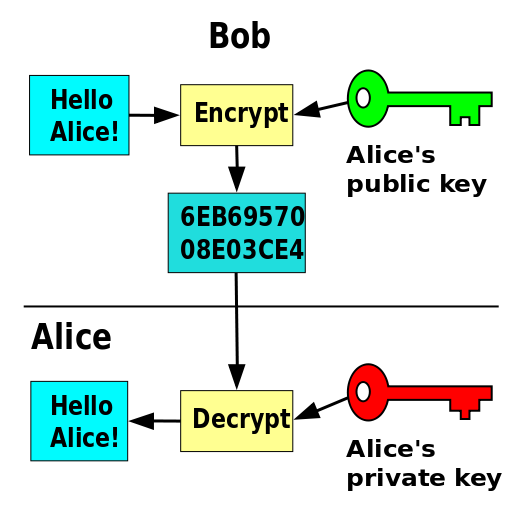
\includegraphics{img/pki-alice-and-bob}
	\centering
	\caption{\gls{PKI} met als voorbeeld Bob die een bericht stuurt naar Alice}
	\label{fig:pki-alice-and-bob}
\end{figure}

Deze toepassing van public key encryption creëert confidentialiteit door het
bericht niet leesbaar te maken voor een 3de partij. Een andere toepassing
hiervan is digitale handtekeningen. Hierbij wordt een bericht ondertekend door
de zender met zijn of haar private sleutel en kan de ontvanger de handtekening
controleren aan de hand van de
publieke sleutel van de verwachte zender. Als de ontvanger deze handtekening
controleert en de controle slaagt, dan betekent dit dat de verzender toegang had
tot de private sleutel en kan er geconcludeerd worden dat de verzender de
eigenaar is van het sleutelpaar. Hierdoor wordt ook verzekerd dat het
bericht niet aangepast geweest is, sinds validatie van een aangepast bericht
niet zal slagen met de originele handtekening.

Deze vorm van encryptie heeft als eigenschap dat elke handtekening gemaakt door
de ene sleutel geverifieerd kan worden door de andere. Dit geldt ook voor
encryptie waar een bericht dat geëncrypteerd is door de ene sleutel, door de
andere sleutel kan worden gedecrypteerd.

Deze vorm van cryptografie is in het algemeen gebaseerd op wiskundige problemen
die nog niet efficiënt kunnen opgelost worden zoals het factoriseren van gehele
getallen. De wiskunde die cryptografie mogelijk maakt ligt echter buiten het
bereik van deze bachelorproef.

\subsection{Compromitatie van een private sleutel}
\label{subsec:comprimitatie-van-een-private-sleutel}
Het compromitteren van een private sleutel leidt tot een algeheel verlies van de
confidentialiteit van alle toekomstige en ooit versleutelde berichten. Het maakt
het ook mogelijk om zowel handtekeningen als versleutelde berichten aan te maken
in naam van de identiteit wiens sleutel werd verloren. Dit maakt het des te
belangrijker om een systeem te hebben waarin sleutels kunnen worden
geïnvalideerd.

\subsection{Verlies van een private sleutel}
\label{subsec:verlies-van-een-private-sleutel}
Het verliezen van een private sleutel verschilt tegenover compromitatie in de
zin dat
de sleutel niet in handen is van een partij met potentiële kwaardaardige
bedoelingen. Hierbij is enkel de mogelijkheid om te handtekeningen en berichten,
die geëncrypteerd zijn met de publieke sleutel, te decrypteren, verloren.

\chapter{Certificaatautoriteiten}
\label{ch:certificaatautoriteiten}

Certificaatautoriteiten bestaan als externe betrouwbare partij om te bewijzen
dat een entiteit en een publieke sleutel aan elkaar gelinkt zijn. Een voorbeeld
hiervan zijn https-certificaten. Deze bevatten onder andere een domeinnaam, een
publieke sleutel en een digitale handtekening van de certificaatautoriteit. Als
een browser verbindt met een server, stuurt deze server een certificaat door
waarna de browser controleert of de domeinnaam op het certificaat overeenkomt
met de site die bezocht wordt en of het certificaat is ondertekend door een
certificaatautoriteit die vertrouwd wordt. Als deze validatie succesvol is, dan
zal de verdere communicatie met de server geëncrypteerd worden met de publieke
sleutel op het certificaat.

\begin{figure}[H]
	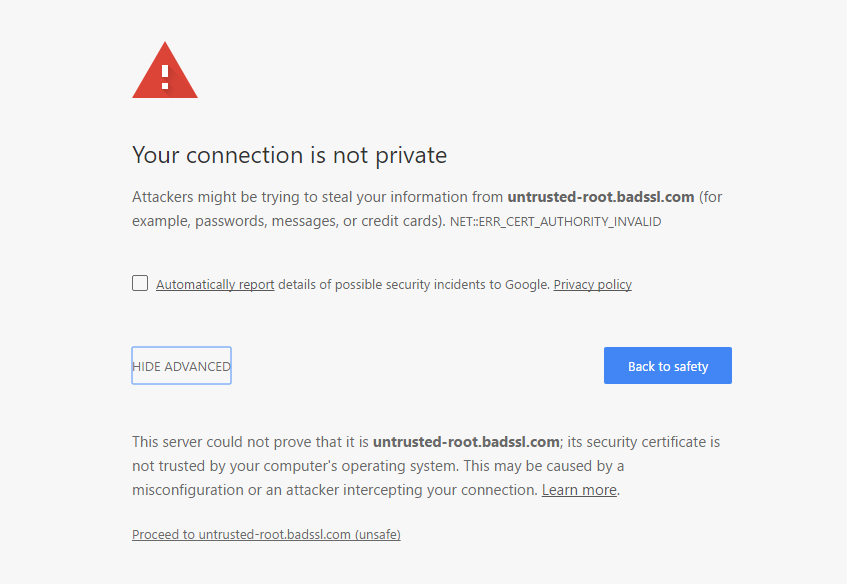
\includegraphics[width=\textwidth,height=\textheight,keepaspectratio]{img/untrusted-root-chrome.png}
	\centering
	\caption{Waarschuwing wanneer een certificaat niet door een certificaat
		autoriteit wordt vertrouwd op Chrome 57.0.2987}
	\label{fig:untrusted-root-chrome}
\end{figure}

\section{Problemen met certificaatautoriteiten}
\label{sec:problemen-met-certificaatautoriteiten}

Het gehele systeem van een vertrouwde derde partij staat en valt bij het juiste
handelen van deze partij. Van elke \gls{CA} wordt verwacht dat zij enkel
certificaten uitreiken aan de geverifieerde eigenaar van een entiteit. Wanneer
een \gls{CA} een
certificaat uitreikt dan zal dit certificaat vertrouwd worden ongeacht de
toestemming van de eigenaar van de entiteit.

Gevallen van onrechtmatige uitgave van certificaten komen voor en deze
certificaten worden actief misbruikt. In augustus 2011 werd vastgesteld dat een
\gls{CA} in Nederland, DigiNotar,
slachtoffer was geworden van een hack waarbij alle acht signing servers waren
gecompromitteerd. Er waren certificaten voor *.google.com gemaakt alsook
certificaten voor Yahoo, Mozilla, WordPress en The Tor Project. In totaal werden
er meer dan 500 certificaten gegenereerd. Het primaire doel van de aanval was
300 000 Iraanse Gmail gebruikers. De Iraanse regering wordt verdacht van het
uitvoeren van de hack. De NSA, de militaire intelligentie organisatie van de
Verenigde Staten, wordt ook verdacht van het inbreken in DigiNotar en het
ongeoorloofd aanmaken van certificaten \autocite{DiginotarNu,
	DigiNotarThreatpost, DigiNotarComputerworld, DigiNotarSchneier,
	DigiNotarTweakers}.

Op 25 juni 2014 gaf een \gls{CA} in India certificaten uit voor 45 Google
domeinen
waarna deze op 2 juli werden ontdekt. Google heeft bijgevolg het volledig
vertrouwen in de certificaatautoriteiten opgezegd \autocite{Wilson2014}.

Verder onregelmatigheden gebeurden met de WoSign \gls{CA} die certificaten
aanmaakte
met de verkeerde uitgavedatums om de restrictie op SHA1 te ontlopen. WoSign
kocht ook een andere \gls{CA} op zonder dit publiek te maken. Een combinatie met
andere gevallen van wangedrag leidde tot het stoppen van het vertrouwen in beide
CAs waarin oude certificaten nog beperkt geldig zullen zijn. Het vertrouwen in
beide CAs wordt volledig uitgefaseerd  \autocite{WoSignMozilla, WoSignTweakers1,
	WoSignTweakers2}.

\chapter{Web of trust}
\label{ch:web-of-trust}

Sinds CAs niet altijd te vertrouwen zijn, ontstond uit de nood voor een
betrouwbaar authenticatie systeem het concept van een web of trust, afgekort
WOT. Dit systeem werkt met een gedecentraliseerd model waarbij niet wordt
vertrouwd op CAs.

Het systeem werkt aan de hand van een soort sleutelhanger waarin alle sleutels
worden opgeslagen. Deze sleutelhanger wordt naar gerefereerd met het woord
‘ring’. Deze ring bevat publieke sleutels van entiteiten. In tegenstelling tot
een centrale autoriteit wordt hier enkel door de beheerder van de ring, sleutels
toegevoegd. De beheerder van de ring beslist ook in hoeverre sleutels vertrouwd
worden.

Een WOT werd ontwikkeld voor \gls{PGP}. Wegens licentieproblemen
werd een nieuwe standaard ontwikkelt die \gls{OpenPGP} werd genoemd. GnuPG is een
gratis implementatie van de \gls{OpenPGP} standaard gemaakt door de Free Software
Foundation. In deze bachelorproef zal, wanneer gesproken wordt van een Web Of
Trust, uitgegaan worden van \gls{OpenPGP} als men spreekt over de standaard en over
\gls{GPG} als over een toepassing wordt gesproken.

Implementaties die conform zijn aan de \gls{OpenPGP} standaard bevatten een
vertrouwensschema. Een sleutel kan de volgende vertrouwensniveaus hebben:

\begin{itemize}
	\item Unknown

	Niets is bekend over het oordeel van de eigenaar van de sleutel in het
	ondertekenen van sleutels.

	\item None

	De eigenaar staat bekend om het incorrect ondertekenen van andere sleutels.

	\item Marginal

	De eigenaar verstaat wat de implicaties zijn van het ondertekenen van een
	sleutel en zal deze vooraf ondertekenen.

	\item Full

	De ondertekening van deze sleutel is even goed als je eigen ondertekening.
	\autocite{GNUManual}
\end{itemize}

Een andere term in de \gls{OpenPGP} standaard is geldigheid. Deze is verschillend van
vertrouwen. Enerzijds is er het vertrouwen in een eigenaar om andere sleutels te
valideren, anderzijds is er de geldigheid van een sleutel. De geldigheid van een
sleutel duidt op het al dan niet vertrouwen dat een sleutel in handen is van de
juiste identiteit.
Dit schema stelt een gebruiker in staat om de identiteit van een sleutel te
verifiëren zonder deze zelf te valideren maar zonder controle te verliezen van
wie deze rechten heeft. Een sleutel die ondertekend is door een sleutel die
volledig vertrouwen geniet zal geldig zijn. Een sleutel die ondertekent is door
drie marginaal vertrouwde sleutels zal ook geldig zijn. Dit aantal kan aangepast
worden zodat een WOT flexibel kan zijn \autocite{GNUManualValidatingKeys}.

\section{Keyservers}
\label{sec:keyservers}

Het verspreiden van je publieke sleutel wordt natuurlijk best gedaan in persoon.
Wanneer het aantal personen waarmee je data uitwisselt toeneemt, wordt dit
moeilijker. Keyservers zijn servers waar je keys van kunt importeren en keys
naar kunt exporteren. Wanneer Alice Bob zijn sleutel ondertekent, dan zal Alice
de ondertekende sleutel exporteren naar een keyserver zodat anderen kunnen zien
dat Alice deze heeft ondertekend. Iedereen kan keys uploaden naar de keyservers
en deze doen zelf geen verificatie van de validiteit of betrouwbaarheid van
sleutels. Verificatie van sleutels is altijd de verantwoordelijkheid van degene
die een sleutel importeert. Er zijn vele keyservers bereikbaar en het merendeel
hiervan synchroniseert met elkaar, het maakt dus niet echt uit naar welke
keyserver je de key uploadt. Sinds keyservers enkel publieke sleutels bijhouden
en deze toch overal bekend mogen zijn, is het ook niet nodig om over een veilig
kanaal je sleutel te uploaden \autocite{GNUManualDistributingKeys}.

Keyservers staan niet toe om sleutels te verwijderen. Dit is om het WOT te
beschermen tegen ongeautoriseerde verwijderingen.

Keyservers hoeven niet per se publiek te zijn. Het is mogelijk om een keyserver
in het interne netwerk van een bedrijf te laten functioneren. Dit soort
keyserver wordt een private keyserver genoemd. Dergelijke private keyservers
bieden het voordeel dat ze niet publiekelijk doorzoekbaar zijn. Hierdoor is het
niet mogelijk om als buitenstaander de e-mailadressen van alle werknemers te
vinden en hierna e-mails te sturen naar e-mailadressen die niet bedoeld zijn om
extern benaderd te worden. Ook geeft dit meer vrijheid aan de beheerders van de
keyserver om sleutels te verwijderen zonder zich zorgen te maken over oude
sleutels die op servers staan waar zij geen toegang tot hebben.

\section{Terugtrekken van sleutels in een Web Of Trust}
\label{sec:terugtrekken-van-sleutels-in-een-wot}

Het verlies van een sleutel en het wachtwoord dat hieraan gelinkt is, heeft tot
gevolg dat eenieder die hier toegang tot heeft, alle data kan decrypteren die
met de publieke sleutel is geëncrypteerd. Verder kunnen digitale handtekeningen
gemaakt worden. Ook bestaat de kans dat entiteiten blijven data encrypteren met de
verloren publieke sleutel die je niet meer kunt decrypteren door een gebrek aan
private sleutel.

Om dit probleem op te lossen bestaat het revocation certificate. Een revocation
certificate kan enkel gegenereerd worden met de private sleutel. Wanneer een
private sleutel verloren is, kan dit certificaat gepubliceerd worden waarmee
wordt tegengegaan dat data wordt geëncrypteerd met de teruggetrokken publieke
sleutel. Decryptie met de private sleutel en validatie van digitale
handtekeningen met de publieke sleutel blijft mogelijk.
\autocite{GNUManualGettingStarted}

Publicatie van een revocation certificate kan door het certificaat te importeren
in een sleutelring en de teruggetrokken sleutel te verzenden naar een keyserver.

\subsection{Designated revokers}
\label{subsec:designated-revokers}

Een andere mogelijkheid die in de \gls{OpenPGP} standaard aanwezig is, zijn designated
revokers. Een designated revoker is een bezitter van een sleutel die een
revocation certificate kan genereren en verspreiden van een andere sleutel.
\autocite{rfc4880} Om een sleutel aan te duiden als designated revoker is het
nodig om toegang te hebben tot de private sleutel en wachtwoord van de sleutel
aan wie de designated revoker zal worden toegewezen. Met andere woorden, het
toewijzen van een designated revoker kan enkel met toestemming van de eigenaar
van de sleutel. Meerdere sleutels kunnen aangewezen worden om de rol van
designated revoker te vervullen. Het toevoegen van een designated revoker is
onomkeerbaar. Dit zorgt voor een ideale mogelijkheid om sleutels terug te
trekken als derde partij zonder dat hiermee mogelijk is om digitale
handtekeningen te maken of berichten te encrypteren en decrypteren in de naam
van de eigenaar van de sleutel.

\subsection{Ontvangen van key revocations}
\label{subsec:ontvangen-van-key-revocations}

Als een persoon zijn revocation certificate uploadt op de keyservers betekend
dit nog niet dat elke correspondent deze herroeping ontvangt. Hiervoor moet de
eigenaar van een ring de sleutels controleren op updates. Dit kan gedaan worden
via het volgende commando \autocite{GnuPGFAQ}.

\begin{lstlisting}[language=bash]
$ gpg --refresh-keys
\end{lstlisting}

Men kan ook een daemon gebruiken zoals parcimonie om de sleutels op de ring te
updaten zonder aan de keyservers te tonen welke sleutels je geïnteresseerd in
bent. Dit systeem werkt via \gls{TOR}. Anonimiteit bij het gebruik van een Web Of
Trust valt echter buiten het domein van deze bachelorproef
\autocite{RiseUpOpenPGPBestPractices}.

\section{Wat kan dit oplossen}
\label{sec:wat-kan-dit-oplossen}

De Web Of Trust implementatie leidt tot het oplossen van \gls{authenticiteit},
\gls{integriteit} en \gls{toerekenbaarheid}. Een identiteit kan bewijzen wie hij of
zij is
door het ondertekenen van data doordat het bezit van de private sleutel en
wachtwoord de authenticatie bevestigd. \Gls{integriteit} van data kan bewezen
worden
door de handtekening van een bericht te valideren. Het ondertekenen van een
bericht of contract kan niet ontkend worden doordat een handtekening enkel
succesvol gevalideerd kan worden via een unieke sleutel en dan de enige persoon
met toegang tot de private sleutel en het wachtwoord hiervan, de eigenaar van de
sleutel is.

Specifiek zou dit het volgende oplossen in het voorbeeldverhaal. Wanneer Thomas
aan Jim beveelt om betaling te verrichten en hij later door heeft dat hij zich
vergist heeft, kan hij niet ontkennen dat hij de betaling aangevraagd heeft. Dit
zuivert Jim van blaam. Hiervoor is echter vereist dat Thomas het bericht waarin
hij de betaling aanvraagt, ondertekend. Het is daarom ook best als alle
communicatie in het bedrijf verplicht standaard digitaal ondertekend zijn.

In het geval dat een impersonator van Thomas probeert om Jim te overtuigen om
een betaling te doen, zal Jim vragen voor een digitaal ondertekend bericht als
bevestiging. Een impersonator zal geen toegang hebben tot de private sleutel van
Thomas en dus geen digitale handtekening kunnen maken hiermee. Dit zou het einde
moeten zijn van deze soort fraude. Indien de impersonator toegang zou hebben tot
de private sleutel van Thomas en het wachtwoord hiervan, dan zijn er zeer grote
consequenties. Het veiligstellen van de sleutels en wachtwoord is een apart
hoofdstuk en wordt later op teruggekomen.


\chapter{Implementatie van een \glsentrytext{GPG} Web Of Trust}
\label{ch:implementatie-van-een-gpg-web-of-trust}

Dit hoofdstuk behandelt hoe een \gls{GPG} Web Of Trust kan worden
geïmplementeerd in
een bedrijf. Onder andere wordt de configuratie van \gls{GPG} onderzocht en
de beste
instellingen geconcludeerd.

\section{Gebruikte algoritmes}
\label{sec:gebruikte-algoritmes}

\gls{GPG} gebruikt meerdere algoritmes om de publieke/private encryptie en
digitale
handtekeningen toe te passen. Het kiezen van het juiste algoritme en de
configuratie hiervan heeft een impact op veiligheid van de sleutels en de
compatibiliteit met andere systemen. We vergelijken de belangrijkste algoritmes
in \gls{GPG}. Het meest gebruikte algoritme is RSA gevolgd door DSA. ECC, wat
staat
voor Elliptic Curve Cryptography, is een nieuwer algoritme dat nog aan
populariteit moet winnen.

RSA is een veelgebruikt asymmetrische crypto en ontleent zijn naam aan zijn
auteurs, zijnde Rivest, Shamir en Adleman. Het gebruik van RSA nam vooral toe
naar het verlopen van het patent in de Verenigde Staten.

DSA, wat staat voor Digital Signature Algorithm, is een variant op het ElGamal
handtekening schema dat ontwikkeld is door de NSA. Het wordt veel gebruikt en
vind het grootste deel van zijn toepassing in oudere toepassingen. DSA vereist
absolute zekerheid van de geheimhouding, willekeurigheid en uniciteit van een
willekeurige waarde. Indien enkele bits van de willekeurige waarde gelekt
werden, kon de private sleutel bepaald worden. Dit bleek uiterst gevaarlijk toen
de NSA een met opzet gebrekkige random number generator publiceerde genaamd
Dual\_EC\_DRBG \autocite{Perlroth2013NsaRng, Zetter2013NsaRng, GuardianNsaRng}.
Het bedrijf genaamd RSA Security, niet te verwarren met het algoritme, dat een
zeer invloedrijke firma is qua computer beveiliging heeft na een betaling van 10
miljoen US-dollar door de NSA, Dual\_EC\_DRBG de standaard gemaakt in zijn
programma, BSafe. Zo werd een beveiligingsbedrijf dat bekend stond om zijn
strijd voor privacy en security de grootste verspreider van deze backdoor
\autocite{Menn2013NsaRsa}.

ECC is nieuwere vorm van public/private key encryption. Het heeft als voordeel
dat de sleutel kleiner is en dat in vergelijking met RSA, kleinere modulus
sleutels nodig zijn om dezelfde veiligheid te bekomen. Een 256 bit ECC-sleutel
staat ongeveer gelijk qua veiligheid aan een 3072 bit RSA-sleutel. Ook is het
aanmaken en verifiëren van digitale handtekeningen sneller.
\autocite{HighSpeedHighSecuritySignatures} Dit is vooral handig op systemen met
een zwakkere processoren zoals Internet Of Things apparaten. Het nadeel van de
implementaties van ECC zoals ECDSA (Elliptic Curve Digital Signature Algorithm)
en Curve 25519 is dat ze nog niet wijdverspreid of nog niet gestandaardiseerd
zijn. Dit zorgt ervoor dat compatibiliteit met andere systemen niet zeker is.

We kunnen concluderen dat tot ECC-implementaties verder uitgewerkt en
gestandaardiseerd zijn, het best is om RSA te gebruiken.

\section{RSA-sleutel bit grootte}
\label{sec:rsa-sleutel-bit-grootte}

De bit grootte van een RSA-sleutel was 512 bits vanaf 1974 tot in de jaren 80.
In de latere jaren 90 werd de aanbevolen grootte verhoogd naar 768 voor
gebruikers en 1024 voor bedrijven \autocite{OriginalRSAKeySizeRecommendations}.
In 2015 publiceerde het \acrshort{NIST} SP 800-57 dat 2048 aanraadt voor
individuen en
apparaten. De grootte van 2048 tot 3072 wordt aangeraden voor, onder andere,
certificaat autoriteiten
\autocite{NISTKeyManagementRecommendationApplicationSpecific}. De 3072 bit
versie wordt aangeraden indien er geen problemen zijn met interoperabiliteit met
andere apparaten. RSA-768 is de grootste modulo die ooit is gefactoriseerd en
publiek bekend is gemaakt \autocite{FactorizationOf768BitRSA}. Dit proces nam
vier jaar in beslag. \textcite{FactorizationOf768BitRSA} voorspeld dat het
factoriseren van een 1024 bit RSA-modulus binnen het bereik ligt van academische
inspanning.

RSA 2048 zou moeten volstaan tot 2030
\autocite{NISTKeyManagementRecommendationGeneral, NISTAlgorithmesAndKeyLengths}.
Hiermee wordt bedoeld dat het technisch niet haalbaar is om een RSA 2048 bit
sleutel te raden. GitHub raad 4096 bits aan
\autocite{GithubGeneratingANewGPGKey}. Het verdubbelen van RSA-bit grootte heeft
echter niet een verdubbeling van de beveiliging tot gevolg. Een RSA 2048 sleutel
geeft 112 bits beveiliging en RSA 2048 geeft ongeveer 140 bits aan beveiliging.
Het verdubbelen van de grootte van de sleutel heeft in vergelijking weinig
invloed op de toegevoegde beveiliging \autocite{GnuPGFAQ}. Een bit grootte boven
2048 wordt dan ook enkel aangeraden als de bijkomende vertraging niet kritiek is
voor de toepassing. Een voorbeeld van een toepassing waar snelheid kritiek is,
is bijvoorbeeld een webservice of website.

\begin{lstlisting}[language=bash, caption={Commando om de snelheid van RSA te
testen}]
$ openssl speed rsa
\end{lstlisting}

Het resultaat van dit commando kan gevonden worden in tabel
\ref{tab:rsa-speed-test}.

\begin{table}[H]
	\centering
	\begin{tabular}{ l | l | l | r | r }
		& \multicolumn{1}{c}{sign} & \multicolumn{1}{c}{verify} &
		\multicolumn{1}{c}{sign/s} & \multicolumn{1}{c}{verify/s} \\
		\hline
		rsa  512 bits & 0.000048s & 0.000004s &  20841.1 & 274224.6 \\
		rsa 1024 bits & 0.000137s & 0.000009s &   7304.4 & 110915.7 \\
		rsa 2048 bits & 0.000624s & 0.000028s &   1603.2 &  36341.9 \\
		rsa 4096 bits & 0.006696s & 0.000100s &    149.3 &   9974.3 \\
	\end{tabular}
	\caption{Snelheid van RSA getest in Ubuntu 16.04, i7-4700HQ (3.4 GHz), 12 GB
		DDR3 1600 MHz RAM}
	\label{tab:rsa-speed-test}
\end{table}

Tabel \ref{tab:rsa-speed-test} kan weergegeven als box plot zoals in grafiek
\ref{fig:rsa-sign-verify-speed-graph}.

\begin{figure}[H]
	\centering
	\begin{tikzpicture}
	\begin{axis}[
		x tick label style={/pgf/number format/1000 sep=},
		ylabel = Aantal milliseconden per bewerking (ms),
		enlargelimits = 0.02,
		legend style={at={(0.5, -0.05)}, anchor=north, legend columns=-1},
		ybar interval=0.8,
		width = \textwidth,
		height = .90\textheight,
		symbolic x coords = {512,1024,2048,4096,8192},
	]
		\addplot
		coordinates {(512, 0.048) (1024, 0.137)
			(2048, 0.624) (4096, 6.696) (8192, 0)};
		\addplot
		coordinates {(512, 0.004) (1024, 0.009)
			(2048, 0.028) (4096, 0.10) (8192, 0)};
		\legend{Sign, Verify}
	\end{axis}
	\end{tikzpicture}
	\caption{Weergave van het aantal milliseconden per ondertekening en
		verificatie
		voor de verschillende bit groottes}
	\label{fig:rsa-sign-verify-speed-graph}
\end{figure}

We kunnen concluderen dat de toegevoegde veiligheid van 4096 bit sleutels in
vergelijking met 2048 bit sleutels niet opweegt tegen het enorme
snelheidsverlies.

\section{Distributie van sleutels}
\label{sec:distributie-van-sleutels}

De distributie van persoonlijke sleutels is een zeer belangrijk aspect van de
veilige werking van het proces. Niemand behalve de eigenaar van de sleutel mag
de sleutel en bijhorende wachtwoord bezitten en enkel het bedrijf mag sleutels
aanduiden als vertrouwd. Ook mag het niet mogelijk zijn om de private sleutel te
onderscheppen met een \textit{Man In The Middle attack}.

In een Web Of Trust is het zo dat elke persoon verantwoordelijk is voor het
identificeren en ondertekenen van de personen met wie hij zal communiceren. Om
te zorgen dat elke nieuwe werknemer zich niet moet persoonlijk identificeren met
elke andere werknemer zou het best zijn als er de mogelijkheid om deze centraal
te kunnen valideren. Het is mogelijk om één centrale sleutel compleet te
vertrouwen of om meerdere centrale sleutels marginaal te vertrouwen. In dit
voorbeeld zullen we één centrale sleutel hebben.

\subsection{De centrale sleutel(s)}
De centrale sleutel vervult de rol van centrale autoriteit. De private centrale
sleutel, O\textsubscript{priv}, wordt beheerd door een medewerker die het volste
vertrouwen van de organisatie geniet. De publieke sleutel is voor iedereen
beschikbaar. Dit kan op verschillende manieren.

Indien alle werkstations onder toezicht van het interne IT departement vallen,
dan kan de publieke sleutel gemakkelijk voorgeïnstalleerd zijn op het
werkstation. Toegang van thuis uit naar de centrale sleutel is niet mogelijk op
deze manier ook als een medewerker zijn of haar eigen toestel gebruikt zal deze
methode tekort komen. Daarom zou het gemakkelijker zijn indien op de website van
het bedrijf, de sleutel beschikbaar is. Deze website zou dan wel moeten
uitgerust zijn met een HTTPS certificaat zodat het niet mogelijk is om deze aan
te passen met een MITM aanval.

\subsection{Bij aankomst van een nieuwe werknemer}
\label{subsec:aankomst-nieuwe-werknemer}
In dit voorbeeld zal Tim, een nieuwe medewerker, geïntroduceerd worden in het
Web Of Trust. Hiervoor worden volgende stappen ondernomen.

\begin{itemize}
	\item Genereren van een eigen sleutelpaar
	\item Centrale publieke sleutel ondertekenen
	\item Centrale sleutel(s) aanduiden als designated revoker
	\item Eigen publieke sleutel verzenden naar de keyserver
	\item Het nieuwe sleutelpaar wordt ondertekend door de centrale sleutel
\end{itemize}

Tim genereert een nieuw sleutelpaar beveiligd met een zelfgekozen, sterk
wachtwoord (zie \fullref{sec:wachtwoordsterkte}). Dit wordt best gedaan via een
programma dat bepaalde eigenschappen zoals bit sterkte en het gebruikte
algoritme, RSA of DSA, afdwingt om zo de soorten sleutels die in het bedrijf
gebruikt worden consistent te houden. Dit zou eventuele problemen met mogelijke
migraties van sleutels naar ID-cards vermijden alsook het verminderen van bugs
in het verwerken van de sleutels met software. Deze software zou namelijk kunnen
verwachten dat de sleutel een RSA sleutel is of geen DSA ondersteunen.
Consistentie is belangrijk.

De sleutel moet natuurlijk ergens worden opgeslagen. Indien de medewerker maar
één werkstation gebruikt, kan de sleutel hierop blijven. Dit is echter bij de
meeste bedrijven niet het geval. Denk maar aan thuiswerk en het gebruik van
smartphones.

Een veelgebruikt medium, namelijk een USB-apparaat, kan hiervoor gebruikt
worden. Om de private sleutel zo veilig mogelijk te bewaren encrypteren we deze
best. Er komt dus nog een laag encryptie bij. Het USB-apparaat kan
gepartitioneerd worden om zowel een geëncrypteerd deel als een niet
geëncrypteerd deel te bevatten. Dit kan handig zijn om publieke sleutels bij te
houden zodat deze gemakkelijk te exporteren zijn en kan dienen om de eigenaar
van de USB te identificeren terwijl de private sleutel veilig bewaard wordt. Dit
wordt aangetoond in figuur \ref{fig:usb-device}.

\begin{figure}[H]
	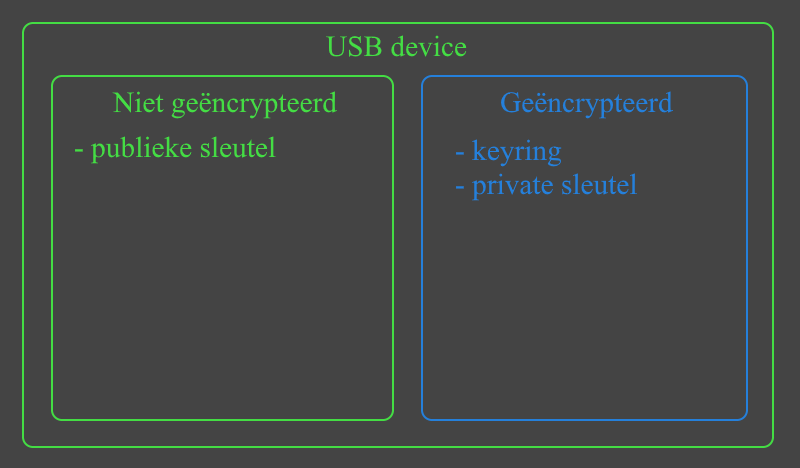
\includegraphics[width=\textwidth,keepaspectratio]{img/usb-store-with-gpg-keys.png}
	\centering
	\caption{USB apparaat waarop de private en publieke sleutel wordt bewaart.}
	\label{fig:usb-device}
\end{figure}

Tim zijn sleutel moet nog gevalideerd worden door de centrale sleutel en vice
versa. De publieke centrale sleutel wordt nu geïmporteerd op het werkstation van
Tim. Deze zou ook voorgeïnstalleerd kunnen zijn. Dit kan via meerdere manieren,
keyservers, USB, … Hierna moet de fingerprint van de sleutel vergeleken en
gevalideerd worden. Nadat dit gebeurd is, ondertekent Tim de publieke centrale
sleutel met zijn sleutel en geeft deze het juiste vertrouwensniveau. Dit zal in
het algemeen marginal of full zijn, afhankelijk van het feit of er meerdere of
één centrale sleutel is. Tim duid de centrale sleutel ook aan als designated
revoker. Hierdoor kan het bedrijf de sleutel terugtrekken indien nodig. Het
proces dat zojuist werd beschreven waarin Tim de centrale sleutel(s) importeert,
kan automatisch gedaan worden door een intern programma dat vooraf
geïnstallleerd was op het werkstation.

De publieke sleutel van Tim moet nu nog geïmporteerd worden in het netwerk van
het bedrijf en ondertekend worden door de centrale sleutel. Dit is nodig omdat
anders andere medewerkers de sleutel van Tim niet zullen vertrouwen. Tim, of het
programma dat de sleutels van de nieuwe medewerkers aanmaakt, geeft hiervoor de
publieke sleutel door aan de beheerder(s) van het centrale netwerk. Hierna
bevestigen Tim en de beheerder(s) van de centrale sleutel dat de fingerprint van
de sleutel overeenkomt. Bij succesvolle vergelijking wordt Tim zijn sleutel
ondertekend door de centrale sleutel en daarna geëxporteerd naar de private
keyserver van het bedrijf. Tim importeert zijn publieke sleutel van de private
keyserver zodat hij de ondertekening van zijn sleutel door de centrale
sleutel(s) lokaal heeft. Deze handeling wordt verricht om te verzekeren dat als
een medewerker de sleutel importeert via het USB apparaat, de ondertekening door
de centrale sleutel(s) direct zichtbaar is. Nu kan Tim aan het werk. Iedereen
die een digitale
handtekening tegenkomt van Tim of wilt communiceren met Tim zal zien dan zijn
sleutel wordt vertrouwd.

Alhoewel Tim aan het werk kan moet er nog een probleem opgelost worden. De
private sleutel bestaat namelijk maar op één plaats. Indien deze verloren raakt,
zal Tim alle data die ooit met zijn publieke sleutel is geëncrypteerd, voor
altijd kwijt zijn. Het is daarom een goed idee om twee USB-apparaten te maken.

\subsection{Online opslag van de private sleutel}
\label{subsec:online-opslag-van-de-private-sleutel}

Het is niet handig om het opslagapparaat overal naartoe mee te nemen. Het
aansluiten met smartphones kan ook een probleem worden indien er geen poort
aanwezig is om het apparaat op aan te sluiten. Om dit op te lossen zou het
mogelijk kunnen zijn om de private sleutel online op te slaan (i.e. cloud) en
deze dan te downloaden wanneer nodig. Er zijn echter bepaalde maatregelen nodig
om zeker te kunnen zijn dat niemand behalve de bezitter van de sleutel, toegang
heeft tot de private sleutel.

De cloud omgeving waarop deze private sleutel wordt opgeslagen moet \textit{zero
knowledge} zijn. Hiermee wordt bedoeld dat de provider van de cloud omgeving
niet in staat mag zijn om de inhoud van de container te lezen. De container in
dit geval is soort map waarin alle geëncrypteerde bestanden zitten. Ook mag een
\textit{Man In The Middle attack} niet resulteren in een gecompromitteerde
private sleutel.

De container mag enkel op het eigen apparaat gedecrypteerd worden. Het
wachtwoord voor decryptie mag het eigen apparaat niet verlaten. Dit voorkomt dat
private sleutel kan bekeken worden door het onderscheppen van de gedecrypteerde
container of het onderscheppen van het wachtwoord. Figuur
\ref{fig:online-zero-knowledge-container} legt uit hoe zo’n systeem kan werken.

\begin{figure}[H]
	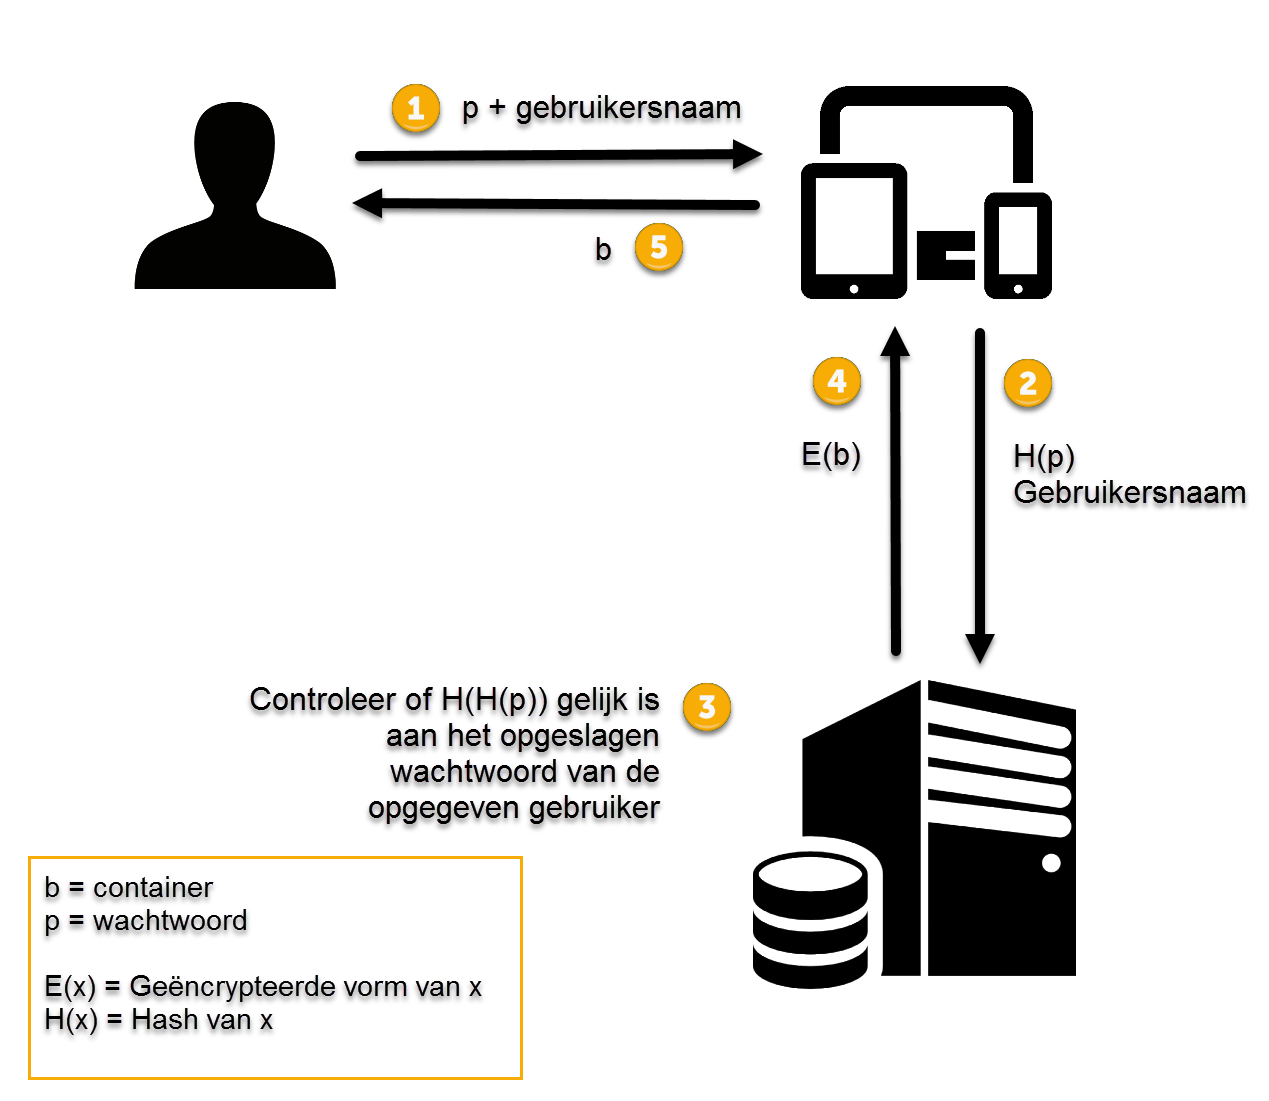
\includegraphics[width=\textwidth,keepaspectratio]{img/encrypted-container-sharing.png}
	\centering
	\caption{Een zero knowledge structuur}
	\label{fig:online-zero-knowledge-container}
\end{figure}

Met deze implementatie verlaat het wachtwoord van de gebruiker, en dus ook het
wachtwoord van de container, het apparaat van de gebruiker niet. Het is sowieso
niet mogelijk om de container te decrypteren zonder het wachtwoord en het
wachtwoord kan niet onderschept worden door een \textit{Man In The Middle
	attack}.

Indien de database met alle gebruikersnamen en wachtwoorden wordt
gecompromitteerd kan een aanvaller nog altijd niet de geëncrypteerde container
buitmaken omdat tijdens de aanmeldpoging het wachtwoord nog eens
\glslink{hash}{gehasht} wordt.
De database bevat namelijk \textit{H(H(p))} en als \textit{H(H(p))} wordt
ingegeven tijdens een aanmelding zal de vergelijking
\textit{H(H(H(p)))~=~H(H(p))} worden. Dit zal natuurlijk een foutieve
aanmeldingspoging tot gevolg
hebben. Alhoewel een aanvaller niets kan doen met de geëncrypteerde container,
zou het succesvol aanmelden op de cloud omgeving tot gevolg kunnen hebben dat de
aanvaller toegang heeft tot een interface waarin containers kunnen beheerd
worden. Hierna zou de aanvaller eventueel een container kunnen verwijderen.

Een dienst zoals dit opzetten vereist een grote kennis van zowel encryptie als
netwerking. Het is daarom niet aangeraden om een dienst zoals dit zelf te maken
zonder de nodige know-how. Er zijn commerciële bedrijven die zo’n dienst
aanbieden, een voorbeeld hiervan is SpiderOak.

\section{Wachtwoordsterkte}
\label{sec:wachtwoordsterkte}

Een belangrijk onderdeel van de sterkte van de encryptie van het opslagapparaat
alsook de sterke van de sleutel is de sterkte van de gekozen wachtwoorden. We
hebben twee wachtwoorden op dit moment, het wachtwoord dat het opslagapparaat
beveiligt en het wachtwoord dat de private sleutel zelf beveiligt. Beide moeten
sterk genoeg zijn om alle soorten van \textit{bruteforce} aanvallen niet
haalbaar te maken.

\begin{figure}[H]
	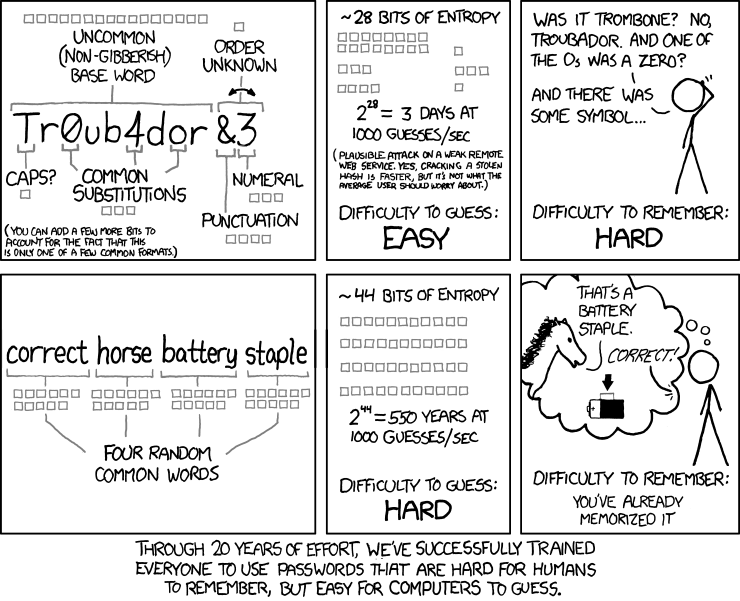
\includegraphics[width=\textwidth,keepaspectratio]{img/password-strength-xkcd.png}
	\centering
	\caption{XKCD: \url{https://xkcd.com/936/}}
	\label{fig:wachtwoord-sterkte-xkcd}
\end{figure}

Figuur \ref{fig:wachtwoord-sterkte-xkcd} toont een bekende XKCD-comic over
wachtwoord sterkte en de wachtwoord vereisten die vaak gevraagd worden.

Uit een voorstel voor een publicatie (zie
\textcite{NISTDigitalIdentityGuidelines}) dat het \acrlong{NIST}, kortweg
\acrshort{NIST}, gepubliceerd heeft betreffende
wachtwoorden en best practices kunnen we enkele zaken concluderen. Wachtwoorden
moeten minstens 8 karakters lang zijn, dit minimum mag verhoogd worden indien
het gaat over gevoelige informatie. Het wachtwoord van de geëncrypteerde
container alsook het wachtwoord van de private sleutel valt hieronder. Een
minimumlengte van 16 karakters moet verplicht worden. Een nog langer wachtwoord
is aangeraden. Wachtwoordzinnen zijn een goede oplossing voor het onthouden van
langere wachtwoorden zoals de XKCD comic (figuur
\ref{fig:wachtwoord-sterkte-xkcd}) ook aangeeft.

Het \acrshort{NIST} zegt verder dat het laten vervallen van wachtwoorden is
afgeraden
aangezien dit de gebruiker niet ten goede komt en kan leiden tot een niet
veilige manier voor het onthouden van het wachtwoord. Een voorbeeld van wat er
kan gebeuren in dit geval is wat er gebeurd is met het Franse tv-kanaal
TV5Monde. In een uitzending werd gefilmd bij een medewerker zijn burea. Op de
muur erachter hingen echter verscheidene notities waaronder wachtwoorden en
gebruikersnaam combinaties \autocite{MachkovechMonde}. Wachtwoorden mogen enkel
vervallen wanneer ze gecompromitteerd zijn.

Wachtwoord tips zijn ten zeerste afgeraden sinds ze teveel kunnen helpen met het
raden van het wachtwoord door aanvallers. Dit gebeurde na de hack van Adobe
waarna 150 miljoen wachtwoorden, gebruikersnamen, en wachtwoordhints werden
buitgemaakt en online gezet. De wachtwoordhints waren zo specifiek dat, door een
combinatie met een slechte \gls{hash}/encryptie methode, een grote hoeveelheid
van de
wachtwoorden herleidbaar was \autocite{HernGuardianAdobeLeak}.

Wachtwoord hergebruik is niet afdwingbaar maar moet sterk afgeraden worden.
Indien hetzelfde wachtwoord gebruikt wordt voor de geëncrypteerde container en
de private sleutel, wordt de veiligheid gehalveerd. Indien een van de
wachtwoorden wordt gebruikt voor een andere service is de veiligheid van het
wachtwoord enkel afhankelijk van de manier waarop deze service met het
wachtwoord omgaat.

\section{Verlies wachtwoord of private sleutel}
\label{sec:verlies-wachtwoord-of-private-sleutel}
Wanneer de mogelijkheid bestaat dat een wachtwoord van een private sleutel
gecompromitteerd is, maar de private sleutel zelf niet, dan moet de eigenaar van
de sleutel een nieuw wachtwoord instellen voor de sleutel. Deze wijziging heeft
enkel effect op de private sleutel. Hierdoor is propagatie in het Web Of Trust
niet nodig.

Indien het wachtwoord van een private sleutel verloren is gegaan, met andere
woorden, de eigenaar van de sleutel is zijn wachtwoord vergeten, of de private
sleutel zelf is mogelijks gecompromitteerd, dan moet de sleutel teruggetrokken
worden. Dit voorkomt dat er misbruik kan gemaakt worden van de sleutel. De
volgende stappen dienen ondernomen te worden. De designated revoker van de
gecompromitteerde sleutel moet zo snel mogelijk op de hoogte gebracht worden. De
designated revoker genereert direct een revocation certificate voor de
gecompromitteerde sleutel. Hierna exporteert de designated revoker dit
revocation certificate naar de keyserver. De \gls{GPG} client die op elk
werkstation
van de werknemers staat, zal tijdens het automatisch verversen van sleutels, het
revocation certificaat binnenhalen. Op deze manier wordt de terugtrekking
doorheen het netwerk gepropageerd.

Afhankelijk van hoe groot de kans is geweest op misbruik, moet gecontroleerd
worden of dit ook het geval geweest is. Dit benadrukt opnieuw het feit dat het
belangrijk is om zo snel mogelijk te reageren om de kans op, onder andere, een
ongewenste handtekening zo klein mogelijk te maken.

Om de werknemer verder te kunnen laten werken moeten de stappen van een nieuwe
werknemer opnieuw uitgevoerd worden (zie subsectie
\fullref{subsec:aankomst-nieuwe-werknemer}). Hetzelfde opslagapparaat kan
gebruikt worden nadat de geëncrypteerde partitie verwijderd is.

\section{Verlies van de geëncrypteerde container}
\label{sec:verlies-geencrypteerde-container}

Het verlies van de geëncrypteerde container is niet ideaal maar betekent niet
dat de private sleutel gecompromitteerd is. Als het wachtwoord van de container
of het wachtwoord van de private sleutel de wachtwoordsterkte vereisten volgt,
dan is het goed mogelijk dat een aanvaller met alle computerkracht in de wereld
er niet in slaagt om het wachtwoord te achterhalen.

Indien er een backup is van de private sleutel dan is het niet nodig om het
sleutelpaar terug te trekken. We vertrouwen immers op de twee lagen encryptie
die ervoor moeten zorgen dat de sleutel niet kan gebruikt worden om e-mails, die
gestuurd zijn naar de betreffende medewerker, te decrypteren. Indien er geen
back-up is zal de designated revoker het sleutelpaar terugtrekken en zal het
proces voor een nieuw sleutelpaar doorlopen worden.

\chapter{Fysieke beveiliging met een Web Of Trust}
\label{ch:fysieke-beveiliging-met-een-wot}

Fysieke beveiliging is het gebruik van fysieke componenten om een plaats,
gebouw, kamer of andere fysieke activa, te beschermen. Fysieke beveiliging kan
gebruik maken van camera’s, bewegingsdetectoren, hangsloten, poorten, deuren en
ook beveiligingspersoneel \autocite{FennellyPhysicalSecurity}. Een Web Of Trust
is gemaakt om de identiteit van een individu te bevestigen en het individu op
manier dan te authenticeren. Voor een toepassing van het Web Of Trust in de
fysieke beveiliging wordt dus gefocust op toestellen of middelen die deze rol
vervullen. Enkele voorbeelden hiervan zijn deuren en poorten.

Toegang restricterende middelen zoals deuren en poorten gebruiken vaak
magneetkaarten, digitale pasjes en soms zelf biometrische eigenschappen zoals
vingerafdrukken van individuen om deze te identificeren. De biometrische
authenticatie heeft als voordeel dat een impersonatie van een individu bijzonder
moeilijk wordt sinds biometrische eigenschappen uniek zijn per individu. De
magneetkaarten en digitale pasjes kunnen daarom ook gecomplementeerd worden met
pincodes of wachtwoorden om de mogelijkheid dat iemand binnen kan met een ander
persoon zijn of haar kaart, te verminderen. De toerekenbaarheid die we moeten
kunnen bewijzen vereist dat als een individu zich authentiseert aan een deur, we
uit de logs moeten kunnen bewijzen dat dit inderdaad door een bepaalde persoon
gedaan was.

Natuurlijk moet elke medewerker niet in alle plaatsen binnen kunnen. Hierdoor is
het vereist dat elke medewerker specifieke toegangsregels kan gegeven worden.

\section{Fysieke toegangscontrole met complementerende beveiliging}
\label{sec:fysieke-toegangscontrole-met-complementerende-beveiliging}

Stel, de private sleutel van de medewerker wordt geplaatst op een elektronische
kaart. De medewerker moet zijn wachtwoord ingeven om het authenticatieproces te
doorlopen. Er zijn direct twee grote problemen met deze aanpak. Het eerste
probleem is dat de private sleutel nu op een ID kaart staat zonder enige vorm
van beveiliging. Wanneer de kaart verloren gaat, is het wachtwoord van de
private sleutel het enige dat het sleutelpaar nog beschermt tegen ongeoorloofde
toegang. Het tweede probleem, is dat het ingeven van een wachtwoord van minstens
zestien tekens en dat complexe karakters kan bevatten zeer tijdrovend zal zijn.

Een betere manier zou zijn om een apart sleutelpaar te gebruiken voor fysieke
toegang. Het wachtwoord dat de private sleutel van dit nieuwe sleutelpaar
beveiligd kan beperkt worden tot getallen. Om duidelijk te maken dat het
sleutelpaar behoort tot een bepaalde medewerker kan deze medewerker de nieuwe
publieke sleutel ondertekenen met zijn of haar huidige sleutel. Deze nieuwe
private sleutel kan dan geplaatst worden op de elektronische kaart waarna bij
authenticatie een toegangsbericht wordt ondertekend bij ingave van het
wachtwoord van de private sleutel. Deze structuur kan teruggevonden worden in
figuur \ref{fig:physical-security-key-structure}. Het authenticatieproces kan
teruggevonden worden in figuur \ref{fig:physical-security-auth-proces}

\begin{figure}[H]
	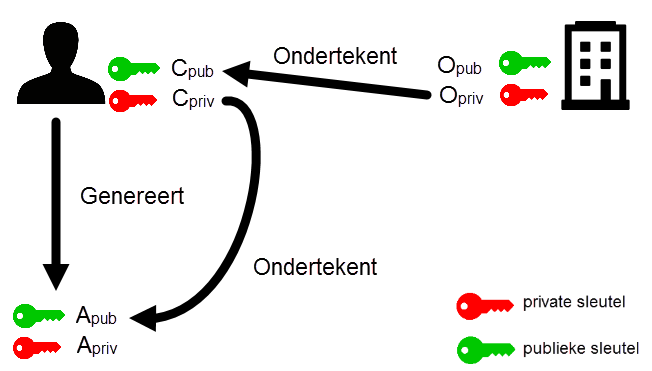
\includegraphics[width=\textwidth,keepaspectratio]{img/physical-security-key-diagram.png}
	\centering
	\caption{Een sleutel structuur met extra persoonlijke sleutel}
	\label{fig:physical-security-key-structure}
\end{figure}

\begin{figure}[H]
	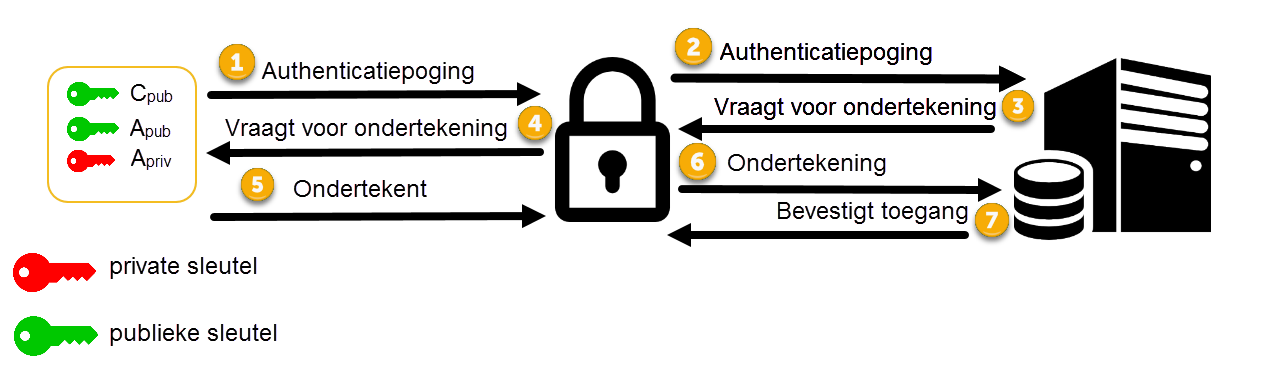
\includegraphics[width=\textwidth,keepaspectratio]{img/physical-security-auth-process.png}
	\centering
	\caption{Een sleutel structuur met extra persoonlijke sleutel}
	\label{fig:physical-security-auth-proces}
\end{figure}

In stap één scant de gebruiker de elektronische kaart. De sleutels op de kaart,
C\textsubscript{pub}, A\textsubscript{pub} en A\textsubscript{priv} worden
doorgestuurd naar de server. De server controleert of C\textsubscript{pub} door
de hoofdsleutel(s) ondertekend is, en de sleutel niet teruggetrokken is.
Vervolgens controleert de server of Apub ondertekent is door het sleutelpaar C.
Indien dit zo is, zal de server een bericht genereren dat een timestamp bevat.
Hierna, in stap drie en vier, zal de server vragen om dit bericht te
ondertekenen. Het individu dat zich nu wilt authenticeren moet zijn of haar PIN
ingeven. De PIN ontgrendelt de private sleutel en ondertekent het gegeven
bericht dat na succesvolle ondertekening na de server wordt teruggestuurd (stap
vijf en zes). In stap zeven controleert de server of de ondertekening correct
is. Indien dit het geval is, betekent dit dat de gebruiker geauthenticeerd is.
Er moet nog een controle gedaan worden op autorisatie. De server controleert nu
of de gebruiker toegang heeft tot de gevraagde plaats. Wanneer dit het geval is
zal de server het toegangsapparaat signaleren om de deur open te doen.

Het is belangrijk om dit te doen nadat het individu geauthenticeerd is. Dit
voorkomt namelijk dat een aanvaller controleert of een bepaalde kaart toegang
heeft tot een plaats zonder een PIN in te geven.

Er is nog één probleem dat moet opgelost worden. De private sleutel wordt
momenteel nog altijd op de badge opgeslagen zonder enige vorm van beveiliging.
Dit betekend dat enkel een PIN de private sleutel beschermt. Een mogelijk
oplossing is een speciaal sleutelpaar aanmaken waarvan de private sleutel op de
access control server staat. De A\textsubscript{priv} sleutel wordt vervolgens
versleuteld met de publieke sleutel van de access control server en
geëncrypteerd opgeslagen op de badge. Bij authenticatie wordt
A\textsubscript{priv} tijdelijk gedecrypteerd voor de handtekening te kunnen
verrichten.

\subsection{Verlies van een badge}

Indien een badge verloren gaat, moet de publieke sleutel die de gebruiker in de
acces control server paart, opgezocht worden en gemarkeerd worden als inactief.
Ook moet het sleutelpaar dat zich op de badge bevond, teruggetrokken worden. De
verloren badge is nu waardeloos voor een potentiële aanvaller. De stappen voor
een nieuwe badge aan te maken worden vervolgens doorlopen.

Indien de badge nog teruggevonden wordt, kan deze leeggemaakt worden en opnieuw
gebruikt.

\section{Fysieke toegangscontrole zonder complementeerde beveiliging}

Het is vaak niet nodig om extra beveiliging zoals PIN of biometrische
authenticatie toe te voegen. Zo’n systeem heeft als voordeel dat er geen tijd
moet worden geïnvesteerd in de extra beveiligingen. Een voorbeeld van een
omgeving waarin dit systeem geprefereerd wordt is bijvoorbeeld een ziekenhuis.
Dit komt door het feit dat in een omgeving zoals een ziekenhuis, snelheid
kritiek is \autocite{Podevyn}. Het aanmaken van dit soort badge staat beschreven
in figuur \ref{fig:electronic-card-creation-no-pin}.

\begin{figure}[H]
	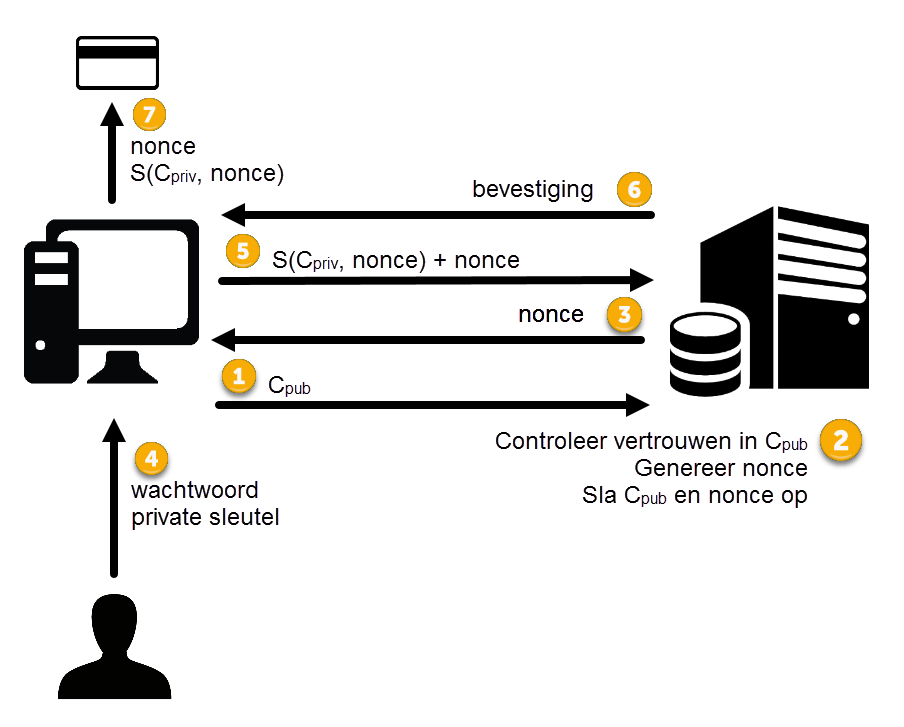
\includegraphics[width=\textwidth,keepaspectratio]{img/electronic-card-creation-no-pin.png}
	\centering
	\caption{Het aanmaken van een ID kaart zonder complementerende beveiliging}
	\label{fig:electronic-card-creation-no-pin}
\end{figure}

Het proces heeft een beginstructuur waarbij de medewerker een badge aangesloten
heeft op de computer waarop hij of zij werkt. De private en publieke sleutel van
de medewerker zijn bereikbaar.

De computer stuurt de publieke sleutel naar de access control server. Deze gaat
na of de publieke sleutel vertrouwd wordt door de hoofdsleutel(s). Hierna
creëert de server een nonce, een unieke willekeurige waarde. De server bewaart
deze nonce samen met de publieke sleutel. Hierna zendt de server de nonce naar
de medewerker zijn of haar computer. De medewerker ondertekent nu de nonce met
zijn of haar private sleutel. Deze bewerking is terug te vinden onder
S(C\textsubscript{priv}, nonce) waarbij S een \textit{sign} methode is, de
eerste parameter gelijk is aan de gebruikte sleutel en de tweede parameter
gelijk aan het bericht. Deze handtekening en nonce worden verstuurd naar de
server. Deze zoekt naar de opgeslagen nonce en valideert de handtekening
vervolgens met de opgeslagen publieke sleutel. Indien deze correct zijn, wordt
dit bevestigt aan het werkstation van de medewerker. Hierna wordt de nonce en de
handtekening ervan op de badge opgeslagen.

Wanneer de medewerker zich authenticeerd bij een fysiek toegang controlerend
systeem, scant hij de badge. De nonce en S(C\textsubscript{priv}, nonce) worden
doorgestuurd naar de server. De server doet een lookup van de nonce. Vervolgens
controleert de server of de publieke sleutel die gevonden is tijdens de lookup,
de S(C\textsubscript{priv}, nonce) kan valideren. Indien dit het geval is, dan
is de medewerker geauthenticeerd. De autorisatie gebeurt op dezelfde manier als
in hoofdstuk
\ref{sec:fysieke-toegangscontrole-met-complementerende-beveiliging}.

\subsection{Verlies van een badge}

Indien een badge verloren gaat, moet de publieke sleutel die de gebruiker in de
acces control server paart, opgezocht worden en gemarkeerd worden als inactief.
De stappen voor een nieuwe badge aan te maken worden vervolgens doorlopen.

Indien de badge nog teruggevonden wordt, kan deze leeggemaakt worden en opnieuw
gebruikt.

\subsection{Voor- en nadelen}
Het voordeel van deze aanpak is dat de private sleutel nooit de veiligheid van
het werkstation van de medewerker verlaat. Het nadeel echter is dat iedereen die
de badge kan bemachtigen, deze kan misbruiken tot het verlies van de kaart
bekend is geworden en er correct naar gehandeld is. Dit wordt gedeeltelijk
gecompenseerd door het feit dat het terugtrekken van de badges minder stappen
vereist.

\section{Access control server}
De access control server heeft als taak om de toegang van alle medewerkers
centraal te beheren. De server heeft enkele gegevens nodig om te kunnen werken.
Hieronder vallen onder andere alle apparaten, deuren, enzovoort die onder access
control vallen. Verder wordt natuurlijk bijgehouden welke personen toegang
hebben welke plaatsen. Een persoon wordt geïdentificeerd aan de hand van een
publieke sleutel.

%...

%%=============================================================================
%% Conclusie
%%=============================================================================

\chapter{Conclusie}
\label{ch:conclusie}

%% TODO: Trek een duidelijke conclusie, in de vorm van een antwoord op de
%% onderzoeksvra(a)g(en). Wat was jouw bijdrage aan het onderzoeksdomein en
%% hoe biedt dit meerwaarde aan het vakgebied/doelgroep? Reflecteer kritisch
%% over het resultaat. Had je deze uitkomst verwacht? Zijn er zaken die nog
%% niet duidelijk zijn? Heeft het onderzoek geleid tot nieuwe vragen die
%% uitnodigen tot verder onderzoek?

Er kan geconcludeerd worden dat een eigen implementatie van een Web Of Trust kan
gebruikt worden om bedrijfsprocessen te beveiligen. Het is echter zeer
belangrijk dat zo'n systeem juist wordt geïmplementeerd.

Een vraag die onbeantwoord is, is hoe data succesvol kan beveiligd worden door
korte of zwakke wachtwoorden. Zou een \textit{lock out} kunnen geïmplementeerd
worden in \gls{GPG}? Het antwoord zou kunnen gebruik maken van een systeem
waarin de kost van een enkele gok naar het wachtwoord te hoog ligt.

Cryptografie zal over de loop van de jaren veranderen, het is daarom verwacht
van de lezer om rekening te houden met de datum waarop deze bachelorproef is
geschreven wannner zaken zoals bit grootte worden besproken. De algoritmen voor
assymetrische encryptie zullen veranderen. \textit{Elliptic curve cryptography}
zal hoogstwaarschijnlijk RSA vervangen. Een eventueele doorbraak van quantum
computing kan het einde betekenen van alle vormen van assymetrische encryptie.
Daarom is het belangrijk, zoals altijd in de IT-wereld, om evolutie in het oog
te houden. Post quantum cryptografie wordt momenteel al onderzocht
\autocite{ANewHopeUsenix}.

Toekomstige ontwikkeling zou eventueel een nieuw decentraal systeem introduceren
of misschien zelf een centraal systeem dat volledig te vertrouwen valt.

Wat betreft de fysieke beveiliging zou het veiliger zijn indien de badge enkel
kon uitgelezen worden door een vertrouwde kaartlezer. Hierbij zou een kaartlezer
zelf ook een sleutelpaar hebben dat ondertekent is door de private sleutel van
de \textit{access control} server. Dit vereist echter dat de badge zelf
berekeningen kan doen. Specifiek zou de badge handtekeningen moeten kunnen
verifiëren. Mogelijks zouden smartphones met NFC technologie hierbij kunnen
helpen.


%%---------- Back matter ------------------------------------------------------

\printbibliography
\addcontentsline{toc}{chapter}{\textcolor{maincolor}{\IfLanguageName{dutch}{Bibliografie}{Bibliography}}}


\listoffigures
\listoftables

\chapter{Bijlagen}

\section{Opmerkingen cryptografisch expert}
\label{sec:opmerkingen-cryptografisch-expert}

"Dit bleek uiterst gevaarlijk toen de NSA een met opzet gebrekkige random
number generator publiceerde genaamd Dual\_EC\_DRBG. -> referentie nodig.
Daarnaast zou je hierover ook eventueel nog iets kunnen zeggen:
\url{http://www.reuters.com/article/us-usa-security-rsa-idUSBRE9BJ1C220131220}

I.v.m. keysterkte, RNG, hashing, kan je met volgende referentie ook helpen:
\url{http://dx.doi.org/10.6028/NIST.SP.800-131Ar1}

Je punt van snelheidsverlies tegenover securitywinst komt duidelijk over. Je
kan echter best wel vermelden welke hardware (op zijn minst het model van de
CPU en het type RAM vermelden) je bij de metingen gebruikt hebt. Dat kan een
rol spelen in verband van reproduceerbaarheid van de resultaten. Tevens ook
vermelden of je een VM gebruikt hebt. VMs hebben namelijk typisch een slechtere
performance op vlak van crypto dan echte hardware.

Ik mis op het einde nog een stukje conclusie m.b.t. de grootte van de sleutels
die je wil gaan gebruiken. Bij \ref{sec:gebruikte-algoritmes} gaf je duidlijk
aan dat "We kunnen  concluderen dat tot ECC-implementaties verder uitgewerkt en
gestandaardiseerd zijn, het best is om RSA te gebruiken.". Zoiets zou hier ook
meerwaarde hebben. Zie bijvoorbeeld opensslspeedtest.txt, waar mijn oude Intel
Core 2 Duo FTPServer het opneemt tegen een mijn Intel Xeon VPS.

Inleiding: hier zou je nog kunnen bijschrijven waarom key distribution zo
kritisch is (MitM natuurlijk).
Inleiding: "Om te zorgen dat elke nieuwe werknemer niet moet persoonlijk zich
identificeren met elke andere werknemer [...]". Ik weet wel dat dat een gevolg
zou zijn van de keuze die je gemaakt hebt voor Web Of Trust, maar dat is voor
de lezer niet direct duidelijk. Ik zou het er expliciet bijzetten.

\subsection{\fullref{subsec:aankomst-nieuwe-werknemer}}

Ik zou hier ook even een kort overzichtje geven met de stappen waardoor een
nieuwe werknemen zal moeten gaan:
1. Keypair genereren;
2. Centrale public key tekenen;
3. Eigen public key naar de server verzenden.

Tim zijn sleutel moet nog gevalideerd worden.  Vermeld erbij vanwaar de
centrale sleutel komt. Wie genereert hem? Waar staat hij opgeslagen? Hoe
verifiëren werknemers dat de cetnrale sleutel die zij op hun scherm zien de
juiste is? Welk medium is het meest betrouwbaar? USB? Misschien hangt de
publieke sleutel ergens op een prikbord? Of misschien kan internal IT de
sleutel mee voorinstalleren bij het prepareren van het werkstation van de
werknemer? Welk medium is praktisch het meest haalbaar? Welke afwegingen maak
je hierbij? Security vs convenience. Ongebruiksvriendelijke security is in de
echte wereld een reëel risico. Tegelijkertijd is gebruiksvriendelijke zwakke
security ook niet optimaal.

Geeft deze het juiste vertrouwensniveau -> Verwijs misschien ook naar hoofdstuk
6, voor meer informatie rond vertrouwensniveau's.

"Het proces dat zojuist werd beschreven waarin Tim de centrale sleutel(s)
importeert, kan automatisch gedaan worden door een intern programma." Tot op
zeker niveau wel. De publieke sleutel zal ofwel in de software ingebakken zijn
(in dat geval verifieert Tim best de hash van de software voor hij die
uitvoert), ofwel zal Tim de fingerprint manueel nog moeten ingeven/verifiëren.

"De publieke sleutel van Tim moet nu nog geïmporteerd worden in het netwerk van
het bedrijf en ondertekend worden door de centrale sleutel." Hierbij vermelden
waarom dat nog moet.

" Tim importeert zijn sleutel van de private keyserver [..]" -> Tim
importeert zijn *publieke* sleutel

Waarom moet Tim lokaal een kopie hebben van
zijn door de server ondertekende sleutel? Volgens mij is dat niet echt
noodzakelijk? Iemand die met Tim wil communiceren kan toch evengoed Tim's
sleutel van de private keyserver afhalen? Zal Tim altijd zijn USB stick moeten
bovenhalen om zijn sleutel te delen? Is het zo onredelijk dat een interne
private keyserver minder te vertrouwen dan een USB stick?

"Het is daarom een goed idee om twee USB-apparaten te maken." Het zou in
ieder geval nuttig zijn om een backup te voorzien. Misschien is het zelfs
handiger om het geëncrypteerde volume van de USB stick binnen het
bedrijfsnetwerk ergens te backuppen? Zo vermijd je de risico's en extra vereise
veiligheidsmaatregelen van de volgende subsection.

\subsection{\fullref{subsec:online-opslag-van-de-private-sleutel}}
"De cloud omgeving moet zero knowledge zijn." Een redelijk grote sprong
tussen dit en de vorige paragraaf. Je zou dat kunnen oplossen door iets hoger:
"private sleutel online op te slaan" -> "private sleutel online (i.e. cloud) op
te slaan". Druk "zero knowledge" best ook cursief.

De term "container" komt hier plotseling op de proppen en wordt vanaf dit
punt nog vaak gebruikt. Deze term heb je nergens geïntroduceerd. Daardoor
onstaat verwarring bij de lezer. Ik zou tussen de eerste en tweede paragraaf
een nieuw paragraafje (of twee) schrijven met wat uitleg in logische volgorde:
- Dat je plant om keypairs in de cloud op te slaan.
- Dat je hiervoor cloud zou kunnen gebruiken of eigen infrastructuur.
- Dat cloud eigenlijk toch wel gemakkelijk is omdat je dan zelf geen
infrastructuur moet aanleggen.
- Het kiezen voor cloud komt met bepaalde risico's: je moet de cloud provider
wel ten zeerste vertrouwen.
- Is er geen andere oplossing dan de cloudprovider te vertrouwen?
- Er bestaat zoiets als encrypted containers, die in principe doen wat Fig 7.2
uitbeeldt (bijv. VeraCrypt).
- Die encrypted containers zou je wel veilig in de cloud kunnen uploaden, mits
Zero Knowledge.
- Wat is zero knowledge?
-> De cloud omgeving moet zero knowledge zijn.

De term "hash" heb je ook nog niet geïntroduceerd. Mogelijk past er wel nog
een kort stukje over one-way functions en hashing in Hoofdstuk
\ref{ch:methodologie}? In dat geval
zou ik hier ook zeker naar H\ref{ch:methodologie} refereren. In dat stukje kan
je bijvoorbeeld de
belangrijkste eigenschappen van goeie hashing functies vermelden (met "voor
meer informatie <literatuur referentie>"). Alsook preimage resistance,
second-preimage resistance, collision attack,...

Merk ook op dat je best ook salt wanneer je hasht.


Ah, nu zie ik waarom je een tweede keer dacht te hashen langs de kant van de
server. Is m.i. nog steeds niet nodig hoor :-) Beschouw bijvoorbeeld een
succesvolle MitM. De aanvaller heeft in dit geval de username en H(p). Stel dat
hij erin slaagt om, op een voor de server legitieme wijze, de gebruikersnaam
van het slachtoffer en H(p) aan te bieden. Dan zal de server de versleutelde
container van de user terugsturen. En wat dan nog? Als H een goede hashing
functie is, en er gesalt is geweest, is de kans dat de aanvaller het wachtwoord
van de user kan berekenen astronomisch klein.
En dan nog... zelfs bij slechtere hashing functies is de kans nog steeds klein.
Beeld je bijvoorbeeld in dat we MD5 zouden gebruiken. De kans op een collision
is hierbij enorm groot. Maar, aangezien de container die je opslaat encrypted
is met AES, ben je met een collision niet veel.
Een voorbeeld: stel, ik versleutel mijn container met AES-128 en beveilig met
de passphrase "mysecretpassword". Veronderstel ook dat MD5("mysecretpassword")
= MD5("md5sucks"). Een aanvaller kan vinden dat MD5("md5sucks") dezelfde MD5
hash geeft als de hash die hij heeft afgeluisterd. Echter, geeft "md5sucks"
geen toegang tot de versleutelde container. Daarvoor heb je "mysecretpassword"
nodig.

Ik zou zeggen, hou beide verhalen in je paper! Wat je al hebt en wat ik hier
zojuist heb neergeschreven biedt zeker een toegevoegde waarde voor een
geïnteresseerde lezer!

Let wel, jouw voorbeeld met een extra hashing biedt geen extra beveiliging in
geval van MitM; enkel wanneer de aanvaller niet weet welke hash je serverside
gebruikt. Dat laatste als assumptie nemen, is tegen het Kerckhoffs principe.
Geen goed idee dus :-)

\subsection{\fullref{sec:wachtwoordsterkte}}
"Wachtwoordzinnen zijn een goede oplossing voor het onthouden van langere
wachtwoorden" -> [...], wat de XKCD comic ook aangeeft.

"Het laten vervallen van wachtwoorden is afgeraden[...]". Hier neem je een
minder conventionele stand in. Voor mij is dat ok, maar je stelt het toch best
iets genuanceerder. Het is nog altijd zo dat eens per 90-180 dagen veranderen
van wachtwoord aanbevolen is en technisch gezien extra beveiliging met zich
meebrengt. Daarentegen is het ook waar dat gebruikers echt niet elke 90-180
dagen moeite willen doen om wachtwoorden van 16 of meer karakters van buiten
leren, en er dan weggetjes rond gaan vinden, zoals je al schrijft. Indien ik de
beslissing moest maken, zou ik eens per jaar van wachtwoord veranderen een
acceptabel compromis vinden.

\subsection{\fullref{sec:verlies-wachtwoord-of-private-sleutel}}
"Om de werknemer verder te kunnen laten werken moeten de stappen van een
nieuwe werknemer opnieuw uitgevoerd worden." -> hier zou ik refereren naar
Sectie \ref{subsec:aankomst-nieuwe-werknemer}

"UTF-16 is 1 112 064" -> realistisch gezien gaan gebruikers maximum 95
verschillende karakters gebruiken (ascii tabel - controle characters), dwz
2\textasciicircum95 (ongeveer 4*10\textasciicircum28) mogelijkheden

\section{Bachelorproefvoorstel}
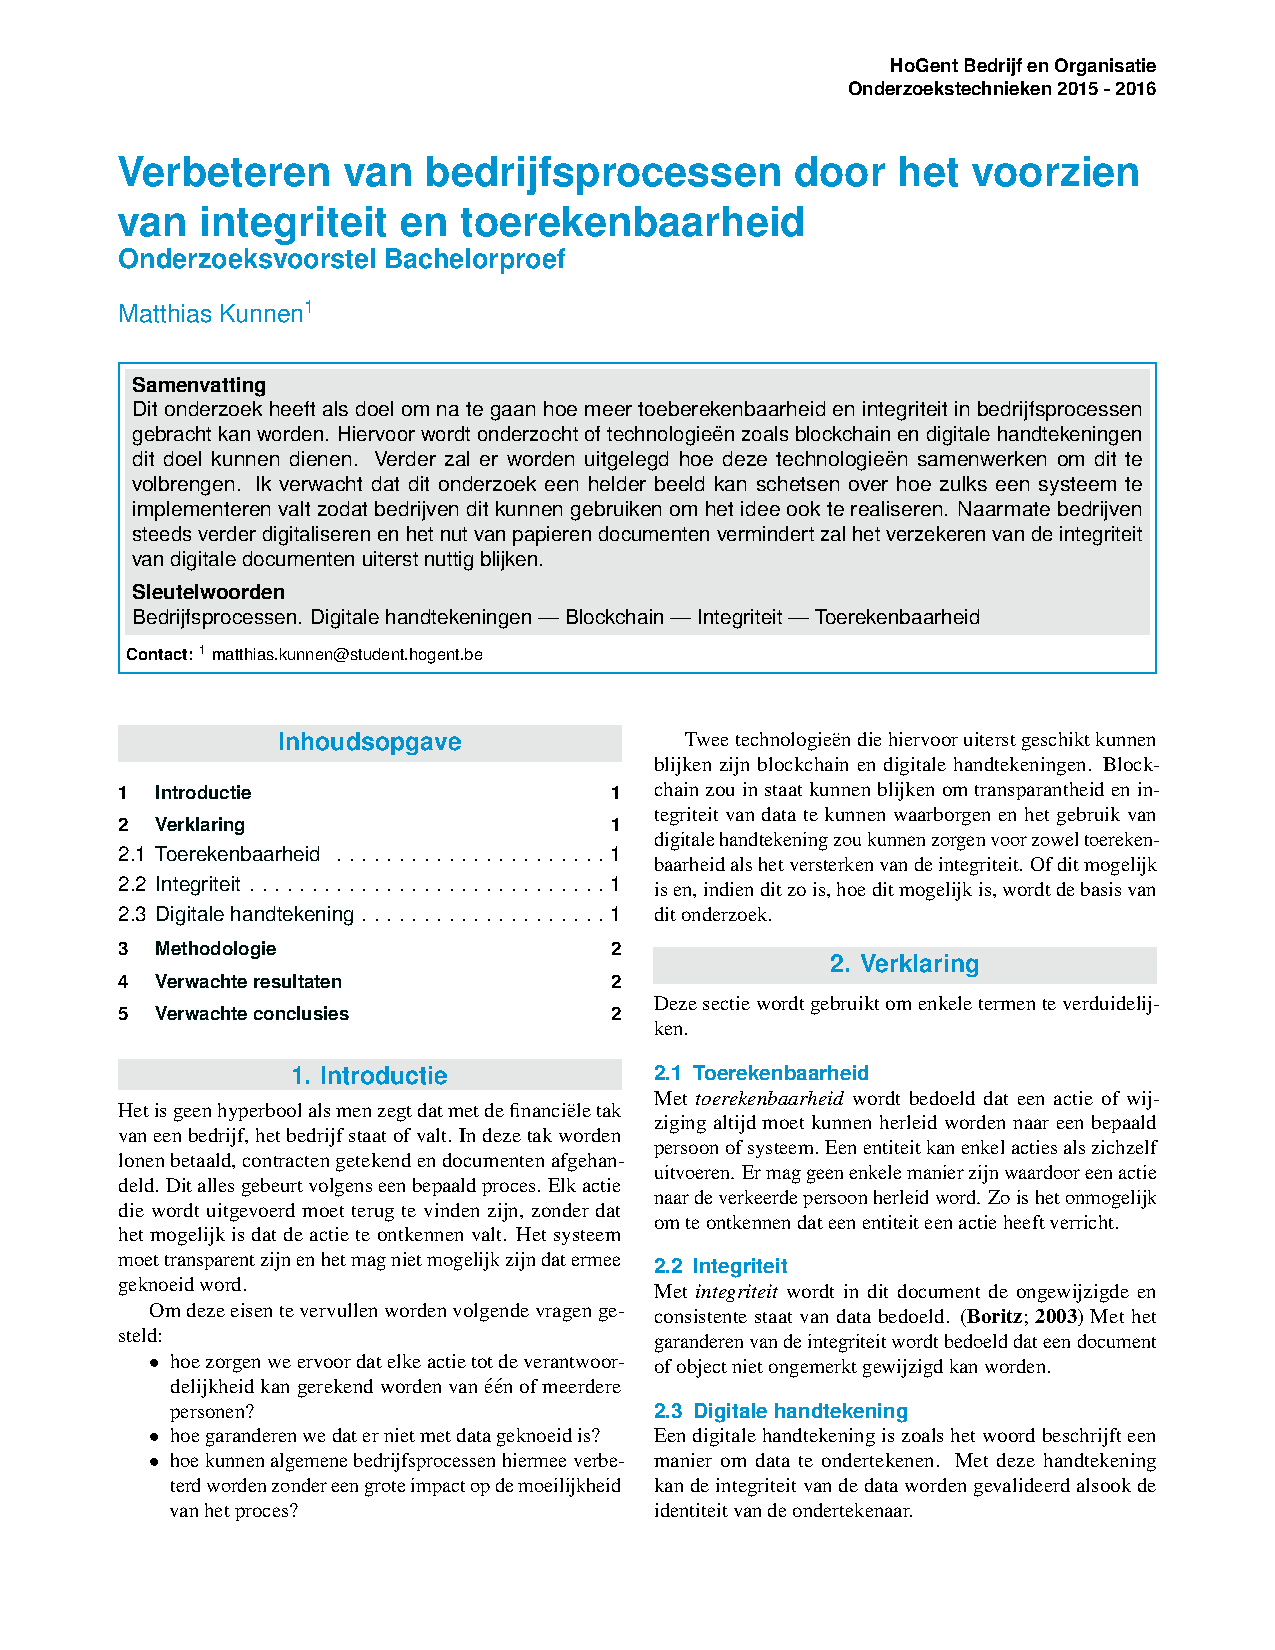
\includepdf[pages={-}]{kunnen-matthias-voorstel.pdf}


\end{document}
